% Template per Elaborato di Laurea
% DISI - Dipartimento di Ingegneria e Scienza dell’Informazione

% formato FRONTE RETRO
\documentclass[epsfig,a4paper,11pt,titlepage,twoside,openany]{book}
\usepackage{epsfig}
\usepackage{plain}
\usepackage{setspace}
\usepackage[paperheight=29.7cm,paperwidth=21cm,outer=1.5cm,inner=2.5cm,top=2cm,bottom=2cm]{geometry} % per definizione layout
\usepackage{titlesec} % per formato custom dei titoli dei capitoli

%%%%%%%%%%%%%%
% supporto lettere accentate
%\usepackage[latin1]{inputenc} % per Windows;
\usepackage[utf8x]{inputenc} % per Linux (richiede il pacchetto unicode);
%\usepackage[applemac]{inputenc} % per Mac.

\singlespacing

\usepackage[english]{babel}

\begin{document}

  % nessuna numerazione
  \pagenumbering{gobble} 
  \pagestyle{plain}

\thispagestyle{empty}

\begin{center}
  \begin{figure}[h!]
    \centerline{
\psfig{file=./chapters/first/marchio_unitrento_colore_it_202002.eps,width=0.6\textwidth}}
  \end{figure}

  \vspace{2 cm} 

  \LARGE{Dipartimento di Ingegneria e Scienza dell’Informazione\\}

  \vspace{1 cm} 
  \Large{Corso di Laurea in\\
  
    Informatica
    %Ingegneria dell'Informazione e delle Comunicazioni
    %Ingegneria dell'Informazione e Organizzazione d'Impresa
    %Ingegneria Elettronica e delle Telecomunicazioni
  }

  \vspace{2 cm} 
  \Large\textsc{Elaborato finale\\} 
  \vspace{1 cm} 
  \Huge\textsc{Titolo\\}
  \Large{\it{Sottotitolo (alcune volte lungo - opzionale)}}


  \vspace{2 cm} 
  \begin{tabular*}{\textwidth}{ c @{\extracolsep{\fill}} c }
  \Large{Supervisore} & \Large{Laureando}\\
  \Large{......}& \Large{Gandelli Alessio}\\
  \end{tabular*}

  \vspace{2 cm} 

  \Large{Anno accademico .../...}
  
\end{center}



  \clearpage
 
  \thispagestyle{empty}

\begin{center}
  {\bf \Huge Ringraziamenti}
\end{center}

\vspace{4cm}


\emph{
  ...thanks to...
}

  \clearpage
  \pagestyle{plain} % nessuna intestazione e pie pagina con numero al centro

  
  % inizio numerazione pagine in numeri arabi
  \mainmatter



    % indice
    \tableofcontents
    \clearpage
    
    
          
    % gruppo per definizone di successione capitoli senza interruzione di pagina
    \begingroup

      \renewcommand{\cleardoublepage}{} 
      %\renewcommand{\clearpage}{} 
    % commentato altrimenti si rompe !!!!!!!!!!!!!!!!!!!!!!!!
      %\titleformat{\chapter}
       % {\normalfont\Huge\bfseries}{\thechapter}{1em}{}
        
      \titlespacing*{\chapter}{0pt}{0.59in}{0.02in}
      \titlespacing*{\section}{0pt}{0.20in}{0.02in}
      \titlespacing*{\subsection}{0pt}{0.10in}{0.02in}
      
      % sommario
      \chapter*{Abstract} % senza numerazione
\label{sommario}
\addcontentsline{toc}{chapter}{Abstract}
% 
We conducted an analysis on the reverts, i.e., when the version of a page is edited or restored to
that of a specific date, made on all the pages and users of Wikipedia in the Italian, Spanish,
Catalan and English versions. We detected specific patterns of reverts such as revert chains: a
series of reverts made by two or more users that continuously delete the previous revert on pages
regarding controversial topics or people. Mutual reverts are instead a pattern that happens when
inside a page two users are both reverting and being reverted by each other. Our goal is to improve
community health by focusing on experienced users. We designed and used state of the art metrics to
detect controversiality based on the revert pattern previously defined. A large portion of the work
was dedicated to the computation of different datasets from the Wikimedia history dumps: having many
small datasets is useful to gather the related data together and to have a faster computation of
them. The datasets generated can be divided into two different modules: chains, containing data
concerning revert chains, and groups, containing data about the different groups the involved users
belong to: admin, registered and anonymous. The last one is useful to classify users as experienced
or not. The generated datasets can be divided into two distinct categories; in the first one, the data
has been saved aggregated by pages, while in the second one by users. The former helps us to have an
idea about those pages in which most of the conflicts takes place and to which topics are related.
The latter is useful to understand how the different groups' activity is distributed on Wikipedia.
The data is saved month by month and this allows us to study the different metrics over time. We
have done a comparative analysis between languages to detect the differences between them. We have
discovered that the percentage of Italian users who have joined a chain is more than three times
higher than in the Catalan and English cases. In the analysis of the admins' influence, it emerged
how in Catalan one half of the reverts are made from admin towards registered users, while in
the Spanish one this value is way smaller. This is also confirmed by the fact that in the Spanish
Wikipedia there are 11 admins per million users versus the 56 in the Catalan one. From the analysis
of the reverts both done and received, we have found an anomaly in the Italian Wikipedia: the
reverts received by anonymous users are in a comparable number with the reverts received by the
registered ones, while in the other Wikipedias we observed how users receive very few reverts. The
analysis of the most controversial topics is also useful to detect sociopolitical issues and track
their development over time. 


\clearpage
\chapter*{Sommario} 
\addcontentsline{toc}{chapter}{Sommario}

Abbiamo condotto un'analisi sui reverts, cioè quando la versione di una pagina viene modificata o
ripristinata a quella di una data specifica, su tutte le pagine e gli utenti di Wikipedia nelle
versioni italiana, spagnola, catalano e inglese. Abbiamo individuato specifici patterns di reverts
come le catene di revert: una serie di revert fatti da due o più utenti che cancellano continuamente
il revert precedente su pagine riguardanti argomenti o persone controverse. I mutual revert sono
invece un pattern che si verifica quando all'interno di una pagina due utenti fanno e subiscono un
revert l'uno con l'altro. Il nostro obiettivo è quello di migliorare la community health
concentrandosi sugli utenti esperti. Abbiamo progettato e utilizzato metriche allo stato dell'arte
per rilevare la controversialità sulla base sui pattern di revert precedentemente definiti. Una gran
parte del lavoro è stata dedicata al calcolo di diversi dataset dal Wikimedia history dumps: avere
molti piccoli dataset è utile per raccogliere i dati tra loro correlati e per avere una velocità di
analisi maggiore. I dataset generati possono essere divisi in due diversi moduli: chains, contenenti
dati riguardo alle catene di revert, e groups, che contengono i dati relativi ai diversi gruppi a
cui appartengono gli utenti coinvolti: admin, registrati e anonimi. Quest'ultimo è utile per
classificare gli utenti come esperti o meno. I dataset generati possono essere divisi in due
categorie distinte; nella prima, i dati sono aggregati per pagina, mentre nel secondo per utente. Il
primo ci aiuta a capire in quali pagine avvengono la maggior parte dei conflitti e a quali argomenti
si riferiscono. Il secondo è utile per capire come è distribuita l'attività dei diversi gruppi di
utenti su Wikipedia. I dati vengono salvati mese per mese e questo ci permette di studiare le
diverse metriche nel tempo. Abbiamo fatto un'analisi comparata tra le lingue per rilevare le
differenze tra di esse. Abbiamo scoperto che la percentuale di utenti italiani che sono in una
catena è più di tre volte più alta che nei casi del catalano e dell'inglese. Nell'analisi
dell'influenza degli amministratori, è emerso come in catalano la metà dei reverts siano fatti dagli
amministratori nei confronti di utenti registrati, mentre in quello spagnolo questo valore è molto più
piccolo. Questo è confermato anche dal fatto che nella Wikipedia spagnola ci siano 11 admin per
milione di utenti contro i 56 di quella catalana. Dall'analisi dei reverts, sia fatti che ricevuti,
abbiamo trovato un'anomalia nella Wikipedia italiana: i revert ricevuti dagli utenti anonimi sono
in numero comparabile con i reverts ricevuti da quelli registrati, mentre nelle altre Wikipedie abbiamo
osservato come gli utenti registrati ricevano pochissimi reverts. L'analisi degli argomenti più
controversi è utile anche per individuare questioni sociopolitiche e tracciare il loro sviluppo nel
tempo. 

% We conducted an analysis on the
% reverts, i.e., when the version of a page is edited or restored to
% that of a specific date, made on all the pages of Wikipedia in Italian, Spanish, Catalan and on part
% of the English one. with the main focus on revert wars, a series of reverts made by two or more
% users that continuously delete the previous revert on pages regarding controversial topics or
% people. By computing datasets containing pages about controversialities, identifed by a metric based
% on the number of reverts, we studied both the revert chains and the groups the users belonged to,
% with the intent to explore the possibility of improving the community health. 

% The works could be devied in two moments, the actual analysis of the datsets and the generations of
% them. Several dataset had been computed from the wikimedia history dumps in order to have small datasets to speed un the
% analysis.The datasets computed could be devided in two different modules: one with the focus on
% revert chains and the other in which we wanted do divide the users in category: admin registered and
% anonymous. each dataset has been computed both by pages and users. 

% Thanks to these data processed we had reach some conclusions, especially doing a comparated analysis
% between languages.

% the data aggregated by pages allow us to understand which are the main controversial topics. the
% data is also saved month by month and this is useful to draw the trend of a page over the time 

% the data aggregated by users helps to identify the volumes of categories of users that perform and
% receive reverts. o to reconstruct the revert history of a user 

% experienced usersok
% community health ok
% controversiality ok
% pattern ok
% mutual reverts ok
% chains ok
% compute datasets 
% revert wars
% conflicts 

      % lista dei capitoli
      \clearpage
      \chapter{Introduction}
Wikipedia  is the biggest source of information currently available on the internet, there are more
than 6 million articles and they are all maintained by volunteers. The value of Wikipedia is all in
the hands of the editors.

Many articles means many users and therefore many potential conflicts. Avoiding these conflicts is
the best way for this encyclopedia to grow. \\ 
Each Wikipedia page has four different sections:  
\begin{itemize}
    \item Article: the actual content of the page.
    \item Talk Page: a forum where people can talk about edits. 
    \item History: a place where everyone can see the older versions of the pages.
    \item Source: in this section users can edit the page. 
\end{itemize}

Conflicts could happen both on the Talk page, through a discussion, and in the Article, through an
edit war. It is valuable to analyze all of these aspects to get a well-rounded view of the problem.

\begin{figure}
    \centering
    
\includegraphics[width=1\textwidth]{./chapters/01/assets/wikipedia_page.png}
    \caption{page structure}
    \label{fig:page}
\end{figure}

\section{Main Project}
\label{sec:Main Project}
The project our team is working on, in collaboration with Eurecat and the Wikimedia Foundation,
is named: “Community Health Metrics: Understanding Editor Drop-off“. this is an excerpt of the
project idea: \\

“The primary value of Wikipedia is the editors. When an editor leaves the project, we lose their
participation and contribution to the community, This could be related to multiple factors, also
external to the project, but it could signal an issue related to internal dynamics and to the health
of the community. While a big effort was dedicated to retain new editors, we lack knowledge and
initiatives focused on understanding and preventing drop-off for experienced editors.”
\\
As stated in the project description, the focus is on expert users, who are the core of Wikipedia:
there are 41,741,926 Wikipedia accounts but active users are only 132,916, namely% of all users

%\footnote{https://stats.wikimedia.org/EN/TablesWikipediansEditsGt5.htm}  %se metto footnote saltano le citazioni 
~ 3\% of all users. 

Focusing on this category of users and understanding the reasons that lead to a drop-off can give a
big help to Wikipedia. Several people are working on this project, this work is just a part of the whole.
In the team, everyone is working on a specific topic with the idea of then merging the different
results to obtain an analysis of the phenomenon from different points of view in order to have a
greater understanding of the life cycle of users.  

The prevention of the drop-off is not the only goal of the project, improving the community health
is also important to let users be in a good environment without being held back from editing. 

\section{My Contribution}
\label{sec:project}
The topic explored in this study is the revert analysis - i.e., when the version of a page is
restored to that of a specific date - for all the articles of Wikipedia.

This project consisted of the analysis of the edit history of different language editions of
Wikipedia to study patterns of reverts and edit wars to understand their potential effect on
individual user activity.

We implemented state-of-the-art metrics of controversy based on reverts and mutual reverts and
developed a new metric based on revert chains. Metrics have been computed per page and per user
monthly.

The results can be viewed in an interactive dashboard available online.

\section{Related Work}
There are several works involving reverts: An interesting tool that allows visualizing conflicts is
the one developed by Suh  \textit{et al.}~\cite{Suh2007}. The problem is that it is from 2007 but Wikipedia started to grow around
2010; now we have new technologies and much more data to analyze so more interesting conclusions can
be reached. There have been analyses of antisocial behavior caused by vandalism~\cite{Kiesel2017}, but since the focus
of the project is on experienced users, this is not relevant to this study. 
      \chapter{Background}
Everyone knows what is Wikipedia and how to read an article, but there are many features
that most people are not aware of, \textit{e.g.} see all the versions of a page and being able to edit it. 
Anyone with a browser and without much effort can see and compare all the edits in a
Wikipedia page. For developers, there are many powerful resources such as big datasets
containing a lot more information.  

\section{History Exploration}
In the history section of a wikipedia article is possibile to see every version of the page.
There are several tools anyone can use to explore the revision history: 
% questa va se vuoi foto e testo vicini
% \begin{wrapfigure}[12]{r}{0.5\textwidth}[h]
%     \centering
%     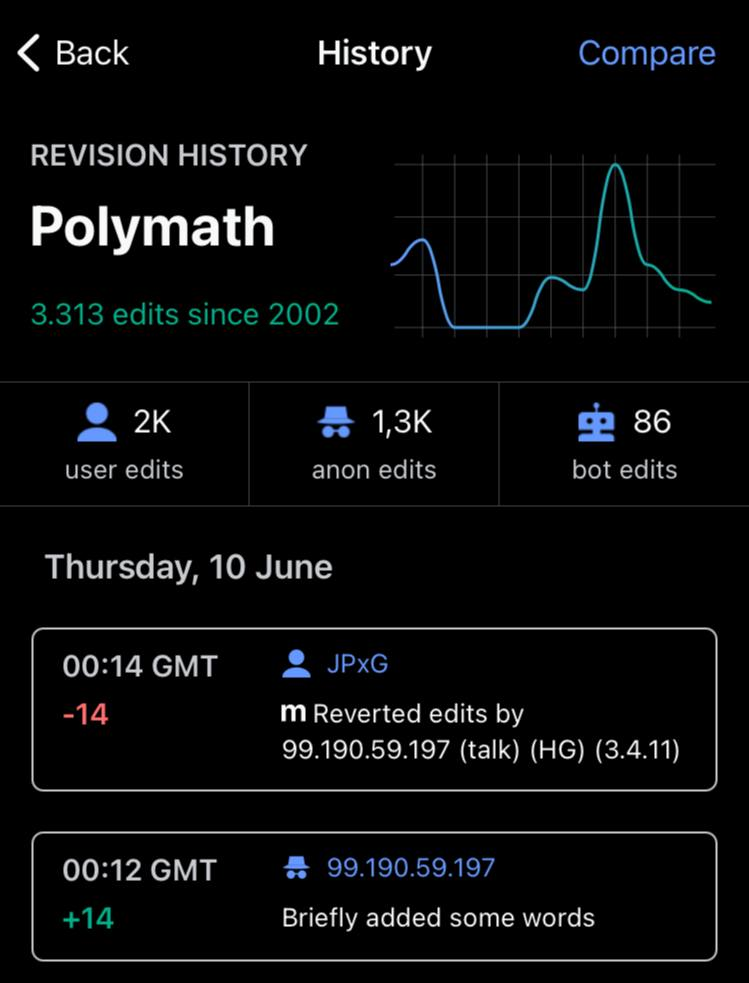
\includegraphics[width=0.35\textwidth]{./chapters/02/assets/mobile_history.jpg}
%     \caption{mobile interactive visualization of the history}
%     \label{fig:mobilehistory}
% \end{wrapfigure}


\begin{itemize}
    \item Mobile application: this resource is only available on mobile device and provides us
        some statistics about the edits of the page like the total number of revisions (Fig \ref{fig:mobilehistory}). 
    \item Website: it is possible to compare two versions with an interactive tool that shows
        the progress of the modified page: each change corresponds to a bar indicating the number of
        bytes added or removed from the revision(Fig. \ref{fig:history}).
\end{itemize}

\begin{figure}[H]
    \centering
    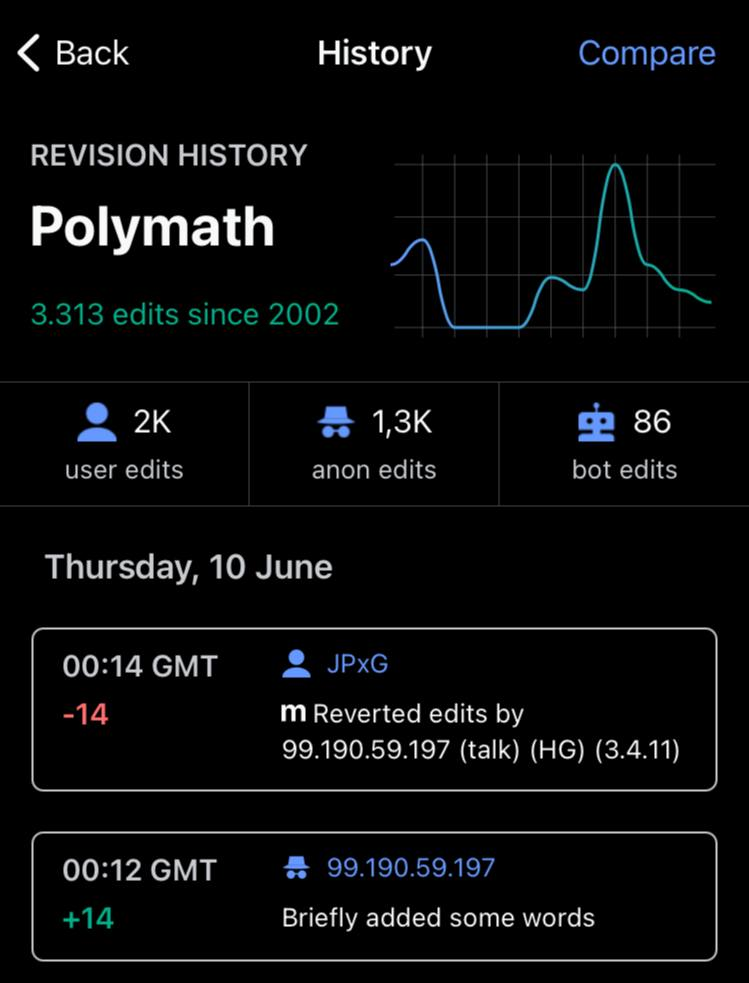
\includegraphics[width=0.35\textwidth]{./chapters/02/assets/mobile_history.jpg}
    \caption{Mobile interactive visualization of the history}
    \label{fig:mobilehistory}
\end{figure}

\begin{figure}[H]
    \centering
    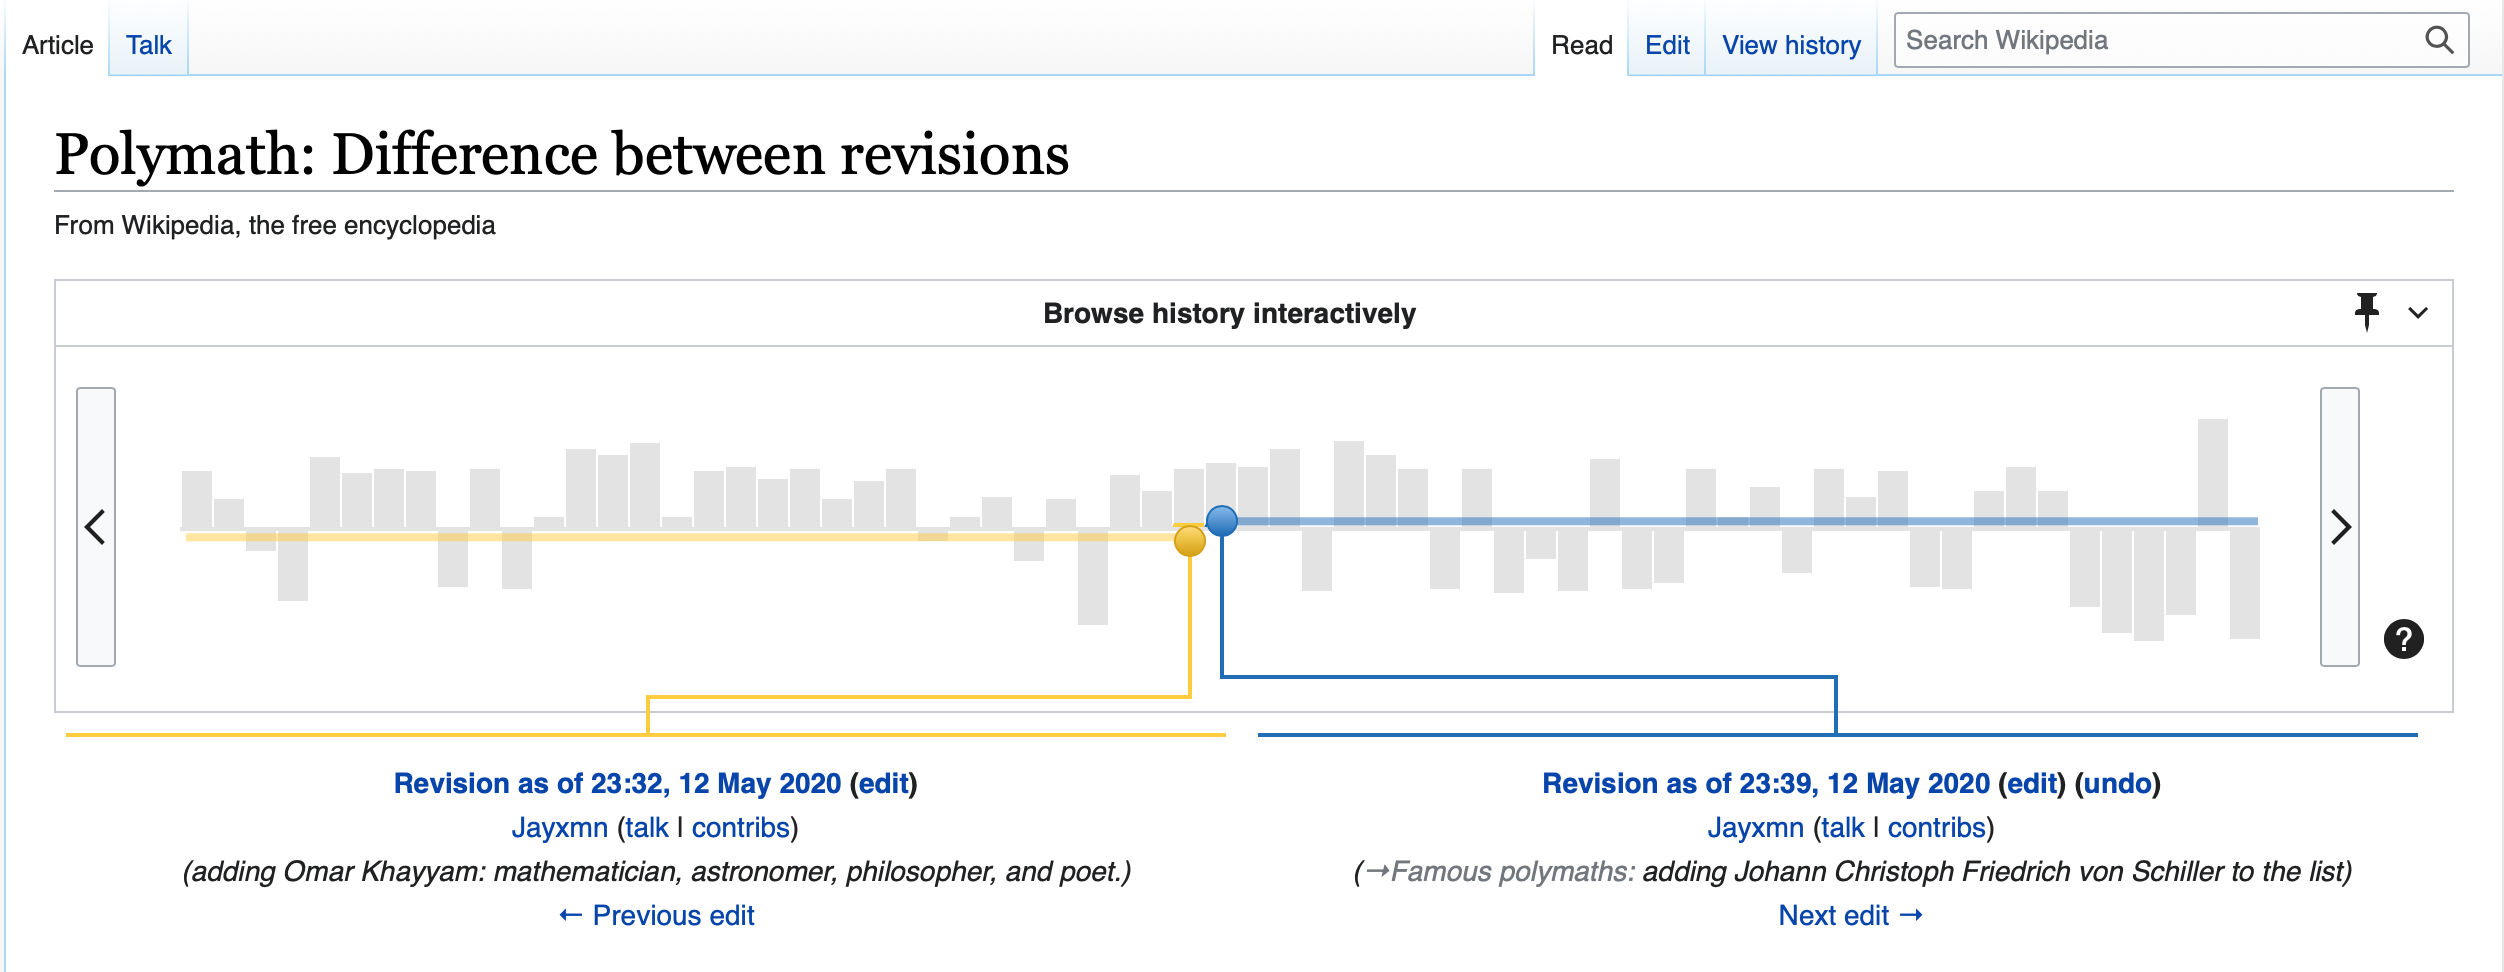
\includegraphics[width=1\textwidth]{./chapters/02/assets/history.png}
    \caption{Interactive visualization of the history}
    \label{fig:history}
\end{figure}


\section{Dataset}
There are two datasets that store info about Wikipedia edits made available from the WikiMedia
Foundation: a) the MediaWiki History and b) the MediaWiki History Dumps


The only difference other than the format (XML the former, TSV the latter) is that the former has the
page content. The dataset used in this study is the MediaWiki History Dumps.\\

Each line of the TSV represent an event and, since it is denormalized, the events for user, page and
revision are stored in the same schema.
All event entity have different event types:
\begin{itemize}
    \item Page: create, delete, move, reatore, merge  
    \item User: create, rename, altergroup (change user rights), alterblocks (block user)
    \item Revision: create (edit a page)
\end{itemize}

In this analysis only revision events are of interest, there are 68 fields but only a few were
needed. The entry could be divided in different sections: one section with general information of
the revision like timestamp and comment, a section with information about the user who did the
revision, one for the page where the revision was made, and the last one with more specific
information about the revision. The most interesting fields of each section are represented in the Tables 
\ref{table:user}, \ref{table:page}, \ref{table:revision}. In the caption are present, if
needed, the descriptions of the fields.

\begin{table}[H]
    \centering
    \ra{1.2}
    \begin{tabularx}{\columnwidth}{@{}Xccccc@{}}
        \midrule
        \textbf{id} & \textbf{username} & \textbf{groups} & \textbf{is\_anonymous} & \textbf{registration} & \textbf{revision\_count}\\ \toprule
        42081 & Checco & autopatrolled & False & 2006-02-10 14:52:44.0 & 10479 \\

         \bottomrule
    \end{tabularx}
    
    \caption{Data about the user who did the revision, the   \textit{groups} field helps to
     identify if the user is an admin, the \textit{revision\_count} is needed to calculate complex metrics like M and G. \label{table:user}}
\end{table}


\begin{table}[H]
    \centering
    \ra{1.2}
    \begin{tabularx}{\columnwidth}{@{}Xccc@{}}
        \midrule
        \textbf{id} & \textbf{title} & \textbf{namespace} & \textbf{revision\_count} \\ \toprule
        116530 & Pino\_Rauti & 0 &  195 
        \\

         \bottomrule
    \end{tabularx}
    
    \caption{Data about about the page where the revision took place,  the \textit{namespace} field is used
    to filter only the revisions because we are only interested in articles, i.e., the actual encyclopedia. \label{table:page}}
\end{table}

\begin{table}[H]
    \centering
    \ra{1.2}
    \begin{tabularx}{\columnwidth}{@{}Xcccc@{}}
        \midrule
        \textbf{id} & \textbf{parent\_id} & \textbf{is\_reverted} & \textbf{reverter\_id} & \textbf{is\_reverter} \\ \toprule
        73507165 & 73506955 & True &  73511400 & False 
        \\

         \bottomrule
    \end{tabularx}
    
    \caption{Data about the revision itself, we are able to identify if the revision is reverting another
    one, if it is been reverted and who is the reverter. \label{table:revision} }
\end{table}


\begin{table}[H]
    \centering
    \ra{1.2}
    \begin{tabularx}{\columnwidth}{@{}Xc@{}}
        \midrule
        \textbf{language} & \textbf{size}\\ \toprule
        English & 540 GB \\
        Spanish & 72 GB \\
        Italian & 54 GB \\
        Catalan & 12 GB \\

         \bottomrule
    \end{tabularx}
    
    \caption{Size of the dataset in different languages. \label{table:datasetsize}}
\end{table}

\section{Definitions}
It is worth defining some terms that will be used several times in the discussion.
\newtheorem{Definition}{Definition}
\begin{Definition}
    (Revert) On Wikipedia, reverting means undoing or otherwise negating the effects of one or more edits,
    which results in the page (or a part of it) being restored to a previous version. % TODO: citare il sito 
\end{Definition}

\begin{Definition}
    (Revert chain) On a Wikipedia page, a revert chain occurs when an edit that reverts an edit is itself reverted.
\end{Definition}

\begin{Definition}
    (Mutual revert) A “mutual revert” is recognized if a pair of editors (x, y) is observed once with x and once with y as the reverter~\cite{Yasseri2014}.
\end{Definition}

\begin{Definition}
    (Editor weight) The weight of an editor x is defined as the number of edits N performed by him or her~\cite{Yasseri2014}.
\end{Definition}

\begin{Definition}
    (Mutual revert weight) The weight of a mutually reverting pair MW is defined as the minimum of the weights of the two editors~\cite{Yasseri2014}.
\end{Definition}

\begin{Definition}
    (Chain weight) The weight of a revert chain CW is defined as the minimum of the weights of the editors involved in the chain.
\end{Definition}


\section{Metrics}
Two complex controversiality metrics have been computed in this study: the first one, M, is the state of the
art metric introduced by Yasseri \textit{et al.}~\cite{Yasseri2014} which give us a score of the controversiality of the page
based on the presence mutual reverts. The second one that we designed, called G, is very similar to M, but
instead of using mutual reverts, it uses revert chains to evaluate the controversiality of the page.  

\paragraph*{Controversiality M}
The controversiality M of an article is defined by summing the weights of all mutually reverting
editor pairs, excluding the topmost pair, and multiplying this number by the total number of editors
E involved in the article.

\begin{equation}
    M = E   \sum_{all\ mutual\ reverts} MW
\end{equation}

\paragraph*{Controversiality G}
The controversiality G of an article is defined by summing the weights off all the chains
there are on a page and multiplying by the total number of editors N involved in at least one chain.

\begin{equation}
    G = N \sum_{all\ revert\ chains} CW
\end{equation}





      \chapter{Methods}

Considering the huge size of the dataset and the fact that a large portion of its content was
useless, smaller datasets have been computed with the aim of expediting the analysis even for future
usages. The analysis was made based on the computed datasets. These datasets can be computed for
every language thanks to a bash script, in this way a multilingual analysis on the most
controversial topics can be conducted in different locations.


\bigskip



\tikzstyle{square} = [rectangle, rounded corners, minimum width=3cm, minimum height=1cm,text centered,text width=3cm, draw=black, fill=blue!20]
\tikzstyle{arrow} = [thick,->,>=stealth]

\begin{tikzpicture}[node distance=4cm]
    \node (dataset) [square, xshift=4cm] {MediaWiki History Dumps};
    \node (computed) [square, right of=dataset, xshift=2cm] {Computed Datasets};
    \node (anal) [square, right of=computed, xshift=2cm] {Analysis};

    \draw [arrow] (dataset) --node[anchor=south] {compute}(computed);
    \draw [arrow] (computed) -- node[anchor=south]{analyze}(anal);

\end{tikzpicture}

\bigskip

\section{Computed Dataset}
After the first skimming, only the revisions involving a revert were saved. This dataset, whose
schema is the same as the MediaWiki History Dumps, has been sorted by both page and timestamp, and
thanks to this screening, the size is now $\sim 10\%$ of the original. In order to achieve this result,
the compressed dataset has been decompressed line by line on the fly and only the entries we were
interested in have been saved in a file. Therefore only a small amount of RAM and disk space is
required since all data is compressed. For the sorting part the most optimized way to sort a file,
which is Unix sort, was used.  

From this filtered dataset several smaller datasets have been computed, and these can be divided into two modules: 

\begin{itemize}
    \item Chains:  the focus was on detecting revert chains in the pages 
    \item Group:  the focus was posed on the number of reverts that users made or received based on the groups they belong to (admin, registered, anonymous).
\end{itemize}

\subsection{Chains}
The data concerning revert chains have been computed from the compressed filtered dataset. Every
time the filtered dataset was analyzed, it was read line by line and only the interesting
pieces of information were saved. The output is a JSON file, in which every page corresponds to a JSON object.
A list of chains and some statistics have been saved for each page. Every chain has a start and an end date, a
list of revisions, and the name of the involved users. The resulting dataset is way smaller than the initial one so it is
possible to browse it in only a few seconds.\\


In order to identify a chain, we used a function, called \textit{simple\_chains}, that differs from
another one, called \textit{complex\_chains} because it identifies a chain of revert only
considering contiguous reverts. We decided to use the simple one because we were only interested in
those chains that occur in a short time span, since there is where most of the discussions take place.
If more than 50\% of users involved in a chain were bots the chain was excluded. There are two
versions of this dataset, one of which considers anonymous users and one that does not. \\

In the schema below there are all the fields in a page object. 
\begin{verbatim}
    {
        "title": "Loligo_vulgaris", 
        "chains": 
        [{
            "revisions": ["113715375", "113715381", "113715393"], 
            "users": {"62.18.117.244": "", "Leo0428": "17181"}, 
            "len": 3, 
            "start": "2020-06-15 22:16:23.0", 
            "end": "2020-06-15 22:17:38.0"
        }], 
        "n_chains": 1, 
        "n_reverts_in_chains": 3, 
        "n_reverts": 38
        "mean": 3.0, 
        "longest": 3, 
        "G": 0,
        "M": 0, 
        "lengths": {"3": 1}
    }
    
\end{verbatim}


The user object is very similar, but it is calculated with another procedure. All the data we needed
was stored in the JSON pages. By analyzing that file all the chains in which a user has been
involved can be extracted, and then statistics can be calculated in a similar way as for pages.
Using this dataset it can be computed 10 times faster.  

The only difference is that the M field is missing because it is only related to a page, while the G field
can be computed on a user considering every chain in which it is the author of at least one revision.\\

The dataset was also computed monthly for both users and pages, the schema is simpler than the
JSON one and this allows us to save it in a TSV using only one row for each month. Instead of saving
all the data regarding the chain, only the numbers of chains longer more than 5, 7, 9 were saved. In
Table \ref{table:chainsPagemonth} there is a sample page entry. In order to do this, the JSON
dataset has been processed one page (or user) at a time, after it was divided by month. The chains
were counted per month basing on the start date of the chain.   

\begin{table}[H]
    \centering
    \ra{1.2}
    \begin{tabularx}{\columnwidth}{@{}Xcccccccccc@{}}
        \midrule
        \textbf{title} & \textbf{year\_month} & \textbf{n of chain} & \textbf{n rev in chain} & \textbf{mean} & \textbf{longest} & \textbf{$\geq$ 5} & \textbf{$\geq$ 7} & \textbf{$\geq$ 9} & \textbf{G}\\ \toprule
        Franz\_Kafka & 2018-11 & 11 & 113 & 10.3 & 51 & 4 & 4 & 3 & 0\\
        
        \bottomrule
    \end{tabularx}
    
    \caption{Entry of the mothly TSV \label{table:chainsPagemonth}}
\end{table}


\subsection{Group}
Another interesting part of this study was focusing on the category a user belongs. Thanks to this
we were able to track the habits of the users, and this can allow us to understand, for example, if
someone stopped editing Wikipedia after several reverts from admins. Detecting these kinds of
patterns is useful for community health. The groups to which users can belong are: 


\begin{itemize}
    \item Admin (sysop): can perform certain actions like blocking users and editing protected pages, 
    \item Registered: are logged in at the time of the edit, 
    \item Anonymous: are not logged in and their username is their IP address(it is not possible to match an IP with a user
        because the IP can change over time).
\end{itemize}

The datasets computed are both for pages and users: 
\paragraph*{Pages} 
For each page, there are two topics of investigation: reverts and mutual reverts. An entry of the
dataset is a page-month containing the number of reverts and mutual reverts made on the page
divided by group. This can be helpful, for example, to detect pages where admins are more active and
this could be a sign that something is wrong with the page.



The notation \textit{adm\_reg} in Table \ref{table:revertpage} refers to the number of admin that performed a
revert to a registered user (similarly with \textit{adm\_adm, reg\_adm, reg\_reg} ).\\

The notation \textit{mut\_ra} in the Table \ref{table:mutualpage} refers to the number of mutual
reverts where the pair is composed by a registered user and an admin. The order of the user does not
matter, in fact, there is no \textit{mut\_ar} that would have the same value.\\


Since the focus was on experienced users, only pairs involving registered and admins were computed.
For having an idea of the volume of the reverts made by anonymous we saved the number of reverts
that were made by both anonymous (\textit{anon}) and not anonymous (\textit{not\_anon}).

To compute these metrics simple variables have been used. They have been incremented, if
necessary, at each entry of the dataset and they have been initialized each time a new page 
started. For both users and pages, we have discarded edits that have been marked as vandalism and
edits made by bots.

\begin{table}[H]
    \centering
    \ra{1.2}
    \begin{tabularx}{\columnwidth}{@{}Xcccccccccc@{}}
        \midrule
        \textbf{id} & \textbf{page} & \textbf{year\_month} & \textbf{adm\_adm} & \textbf{adm\_reg} & \textbf{reg\_adm} & \textbf{reg\_reg} & \textbf{anon} & \textbf{not\_anon}\\ \toprule
        1 & AS\_Roma & 2020-10 & 14 & 245 & 36 & 308 & 1493 & 603 \\
        
         \bottomrule
    \end{tabularx}
    
    \caption{Entry of the revert page TSV. \label{table:revertpage}}
\end{table}

Mutual reverts are not as easy to compute as reverts. We need to store information of the whole page
in order to correctly detect all the mutual reverts.

The most efficient way to save such information is using dictionaries. For each reverter has been
saved the list of users who reverted. At the time of processing the page the saved information
allowed us to compute mutual revert pairs.

\begin{table}[H]
    \centering
    \ra{1.2}
    \begin{tabularx}{\columnwidth}{@{}Xcccccccc@{}}
        \midrule
        \textbf{id} & \textbf{page} & \textbf{year\_month} & \textbf{M}& \textbf{mut\_aa} & \textbf{mut\_ra}  & \textbf{mut\_rr} & \textbf{anon} & \textbf{not\_anon}\\ \toprule
        1 & Giorgio\_Napolitano & 2020-07 & 7681159 & 0 & 4  & 3 & 61 & 7 \\
         \bottomrule
    \end{tabularx}
    
    \caption{Entry of the mutual revert page TSV. \label{table:mutualpage}}
\end{table}

\paragraph*{User}
It is useful also to have the data aggregated by user. Reverts data can be retrieved from the
filtered dataset sorted by timestamp. The data about reverts is gathered and processed month by
month. We store, for each user-month, the number of reverts made and received divided by group.

When a user performs a revert, thanks to the Wikimedia History Dumps, we can know the id of the
revision which is reverting but not the id of the reverted user. To solve this problem we
had to save the info in different dictionaries: \textit{reverters, editor, groups}, 
\bigskip

reverters[username] gives us the list of the revision it reverted. \\
\indent editor[revision\_id] gives us the user who performs that edit. \\
\indent groups[username] gives us the groups a user belongs.\\

Combining this dictionaries we have all the data necessary to compute all the metrics we need.
\begin{table}[H]
    \centering
    \ra{1.2}
    \begin{tabularx}{\columnwidth}{@{}ccc@{}}
        \midrule
        \textbf{user} & \textbf{group} & \textbf{year\_month} \\ \toprule
        carlos & adm & 2020-10  \\
        
         \bottomrule
    \end{tabularx}
    \begin{tabularx}{\columnwidth}{@{}XXXXXXXX@{}}
        \midrule
        \textbf{received} & \textbf{r\_reg}  & \textbf{r\_not} & \textbf{r\_adm} & \textbf{done} & \textbf{d\_reg} & \textbf{d\_not} & \textbf{d\_adm}\\ \toprule
        13 & 12 & 42  & 0 & 13 & 12 & 42  & 0  \\
        
         \bottomrule
    \end{tabularx}
    
    \caption{Entry of the mutual user TSV. \label{table:revks}}
\end{table}


The mutual revert analysis was harder to implement because in order to save the information about
mutual reverts we need the dataset sorted by pages, but to get the data monthly we should use the
one sorted by timestamp. We solved this problem by storing the user-page-month in the dataset, i.e.,
the information about the mutual reverts of a user in a specific month on a specific page.
This led to a larger dataset but with a higher level of information: it is easy to post-process it
grouping by user or month to have one entry per user or one entry per month, respectively. 


\begin{table}[H]
    \centering
    \ra{1.2}
    \begin{tabularx}{\columnwidth}{@{}XXXXXXX@{}}
        \midrule
        \textbf{user} & \textbf{group} & \textbf{page\_name}& \textbf{year\_month} & \textbf{mut\_adm}& \textbf{mut\_reg}& \textbf{mut\_not}\\ \toprule
        khalu & adm & Barcelona & 2020-10 & 13 & 12 & 4 \\
        
         \bottomrule
    \end{tabularx}

    
    \caption{Entry of the mutual user TSV. \label{table:rjevks}}
\end{table}








      \chapter{Results and Discussion}

The second step of this work was the analysis of the generated datasets. Thanks to the structure
and the heavy pruning the analysis of these datasets was fast, this allowed us to have a better workflow
without any interruption. We analyzed the data in two ways: a descriptive statistic and an interactive
one.
\paragraph*{Descriptive}
For each dataset, there is a script that plots various statistics using the python libraries
Pandas and Matplotlib. There are two types of output: plots and rankings. 
Plots are useful to understand the trend from a more comprehensive point of view and on a monthly base.  
Rankings are instead used to see the pages/users ordered in a more specific way by one of the
metrics previously computed. 
\paragraph*{Interactive}
We decided to make an interactive dashboard available online. The idea is
that everyone can change a few parameters and see how the metrics are performing in a personalized
way. To achieve this we uploaded our dataset on a database and thanks to an innovative way to retrieve
data (grapQL) we can display it on a website. 

\paragraph*{Generic statistics }
As we can see here the biggest part of the pages has 0 reverts. Since filtering the Wikimedia
History Dumps removed all the pages with 0 reverts, this field has been computed by subtracting, from the
total number of pages, a value that is available on Wikipedia \footnote{\url{https://en.wikipedia.org/wiki/Special:Statistics}}.

\begin{table}[H]
    \centering
    \ra{1.2}
    \begin{tabularx}{\columnwidth}{@{}Xll@{}}
        \midrule
        \textbf{n\_reverts} & \textbf{n\_pages\_it} & \textbf{n\_pages\_ca}  \\ \toprule
        0 & 1.296.915& 626,5326\\
        1   & 186,539& 32,233 \\
        2-4 & 122,072& 15,387 \\
        5-9 & 45,391& 4,791 \\
        10-99 & 47,833& 3,906 \\
        100-999 & 4,145& 84\\

        \bottomrule
    \end{tabularx}
    
    \caption{Number of reverts for Italian and Catalan Wikipedia. \label{table:pagesmorechains}}
\end{table}
\section{Chains}
Thanks to the analysis of the page chains we can have an overview of an entire Wikipedia in a
language, discovering statistics like the mean length of chains or the longest one. Another aspect
worth investigating was the relationship between solitary reverts and reverts that are in a chain: more
reverts in chains mean more discussions. In cases like these combining the data of the other team
members who analyzed the talk pages could be useful to better understand the dynamics. While the chains in
the pages are useful to have a less specific but wider view of the phenomenon, studying the chains a
user joined lets us see if a specific user is involved in many chains and in which pages is more
active. In this sense, we can define different categories of users: the ones who are active just in
some topic or the others who revert on all Wikipedia. \\

Monthly metrics are even more interesting: we can plot the trend of reverts on a page and see if it
is always controversial or just in a specific historical moment related to something that happened
in the world. Plotting the metrics year by year allows us to understand the global activity of the
users on Wikipedia. We can define the lifecycle of a user and see when it is more active, and if
its decrease of revisions is related to a discussion.\\


In Table \ref{table:generalstats} there is an overview of the number of solitary reverts and
reverts which belong to a chain in the Wikipedia of different languages. The ratio between the
number of reverts that are in a chain and the ones that are not is a useful indicator of how much
the users are committed. In the Catalan Wikipedia this ratio is higher and we could refer this to
the patriotism that brought more attention on certain topics that we will explore later in Table
\ref{table:morechains}.

\begin{table}[H]
    \centering
    \ra{1.2}
    \begin{tabularx}{\columnwidth}{@{}Xrrrrr@{}}
        \midrule
        \textbf{len}& \textbf{revisions} & \textbf{reverts} & \textbf{reverts on edits} & \textbf{reverts in chain} & \textbf{\% in chain} \\ \toprule
        en &1,027,188,756&66,147,314&6.4\%&6,144,948& 10\%\\
        es &136,318,137& 11,539,552&8.4\%& 1,065,618 & 9\% \\
        it &121,362,136& 7,712,039 &6.4\% & 850,020 &  11\% \\
        ca &27,657,030& 355,251 & 1.3\%& 56,280 & 15\% \\
    
        \bottomrule
    \end{tabularx}
    
    \caption{Number of reverts in Wikipedia in Spanish, Italian, and Catalan. \label{table:generalstats}}
\end{table}


\subsection{Page}
In Table \ref{table:morechains} the pages are ranked by the number of chains in Italian, Catalan,
and Spanish. In the Italian one six out of ten pages were football-related while in the catalan one
we can see, as expected, a stronger territorial belonging, the Spanish ranking tells us that the
main part of Spanish Wikipedia users are from Latin America and that they are interested in
football. It is interesting to note how in the Catalan Wikipedia the second surname of the person which the
article is about is written in the title of the article while in the Spanish one it is not.
\begin{table}[H]
    \centering
    \ra{1.2}
    \begin{tabularx}{\columnwidth}{@{}Xllllll@{}}
        \midrule
        \textbf{id} & \textbf{title} & \textbf{chains}& \textbf{title} & \textbf{chains} & \textbf{title} & \textbf{chains} \\ \toprule
        1 & Serie A & 195  & Barcelona & 68 & Club América & 222\\
        2 & Juventus FC & 190  & FC Barcelona & 33 & Deporte en Argentina & 218\\
        3 & Matteo Renzi & 179  & Catalunya & 30 & Club Universitario & 213\\
        4 & AS Roma & 176  &País Valencià& 26 & Club Guadalajara & 211\\
        5 & Personale WWE & 167  &Marc Márquez i Alentà & 22 & América Latina & 185\\
        6 & SSC Napoli & 162  & Mireia Belmonte i García& 22 & Club Alianza Lima & 179\\
        7 & Inter  & 162  &Girona & 20 & Idioma español & 171\\
        8 & Roma & 154 & Rafael Nadal i Parera & 19 & Juventus de Turín & 162\\
        9 & Tiziano Ferro & 141 & Oriol Junqueras i Vies& 17 & Ecuador & 160\\
        10 & Gianluigi Buffon & 137  &Català & 16 & Bogotá & 159\\
        
         \bottomrule
    \end{tabularx}
    
    \caption{Pages with more chains \label{table:morechains}}
\end{table}


In the analysis of the longest chain, the scenario we face is different. The top topics are not
sports but cinema, music and literature for Italian. But here the most fascinating things happen on
the Catalan Wikipedia: we can see how the longest chains are all related to Navarra, doing a more
specific research we can see that it is all related to the language used to identify cities, this is
probably vandalism from some Spanish user who wanted to suppress the Basque language. These metrics
cannot be used for detect problems in the community health but can let some sociopolitical
issues inside a place with linguistic minorities emerge.
\begin{table}[H]
    \centering
    \ra{1.2}
    \begin{tabularx}{\columnwidth}{@{}Xllllll@{}}
        \midrule
        \textbf{id} & \textbf{title} & \textbf{longest it}& \textbf{title} & \textbf{longest ca} & \textbf{title} & \textbf{longest es} \\ \toprule
        1 & Pino Rauti  & 114  & Roncal-Salazar & 81 & Alan  Jackson & 178\\
        2 & Carlos Tévez & 66  & Tractat  d'Utrecht & 80 & A & 172\\
        3 & Rogue  One & 64  & Gazteluberri & 76 & Consejo  Mundial  de  Boxeo & 140\\
        4 & Rocky  Marciano & 64  &Comarca  de  Sangüesa& 71 & Guerra  anglo-española  (1625-1630) & 140\\
        5 & Poeta  urbano & 58  &Comarca  d'Aoiz & 69 & Guerra  de  la  Independencia  Española& 137\\
        6 & Paradisi  per  illusi & 55  & Comarca  de  Lumbier& 69 & Guerra  anglo-española  (1585-1604) & 121\\
        7 & Kuromajo-san  ga  toru!  & 53  &Riu  Gor & 53 & Independencia  de  la  República  Dominicana & 107\\
        8 & Matt  Dillo & 52 & Tudela & 51 & Kreutzberger & 100\\
        9 & Aletheia  (album) & 52 & Igúzquiza& 50 & Dalas  Review & 99\\
        10 & Franz  Kafka & 51  &Untziti & 48 & Bastille & 96\\


         \bottomrule
    \end{tabularx}
    
    \caption{Pages sorted by longest chains. \label{table:longestchain}}
\end{table}


\paragraph*{monthly}
By analyzing the trend(Fig \ref{fig:chainsuser}) of the page (Barcelona in Catalan) we can clearly
see that even if there are a lot of chains the controversiality metric G grows mainly on one
occasion, the reason is that in that chain experienced users are involved so this metric is useful
to detect discussion between them.
\begin{figure}[H]
    \centering
    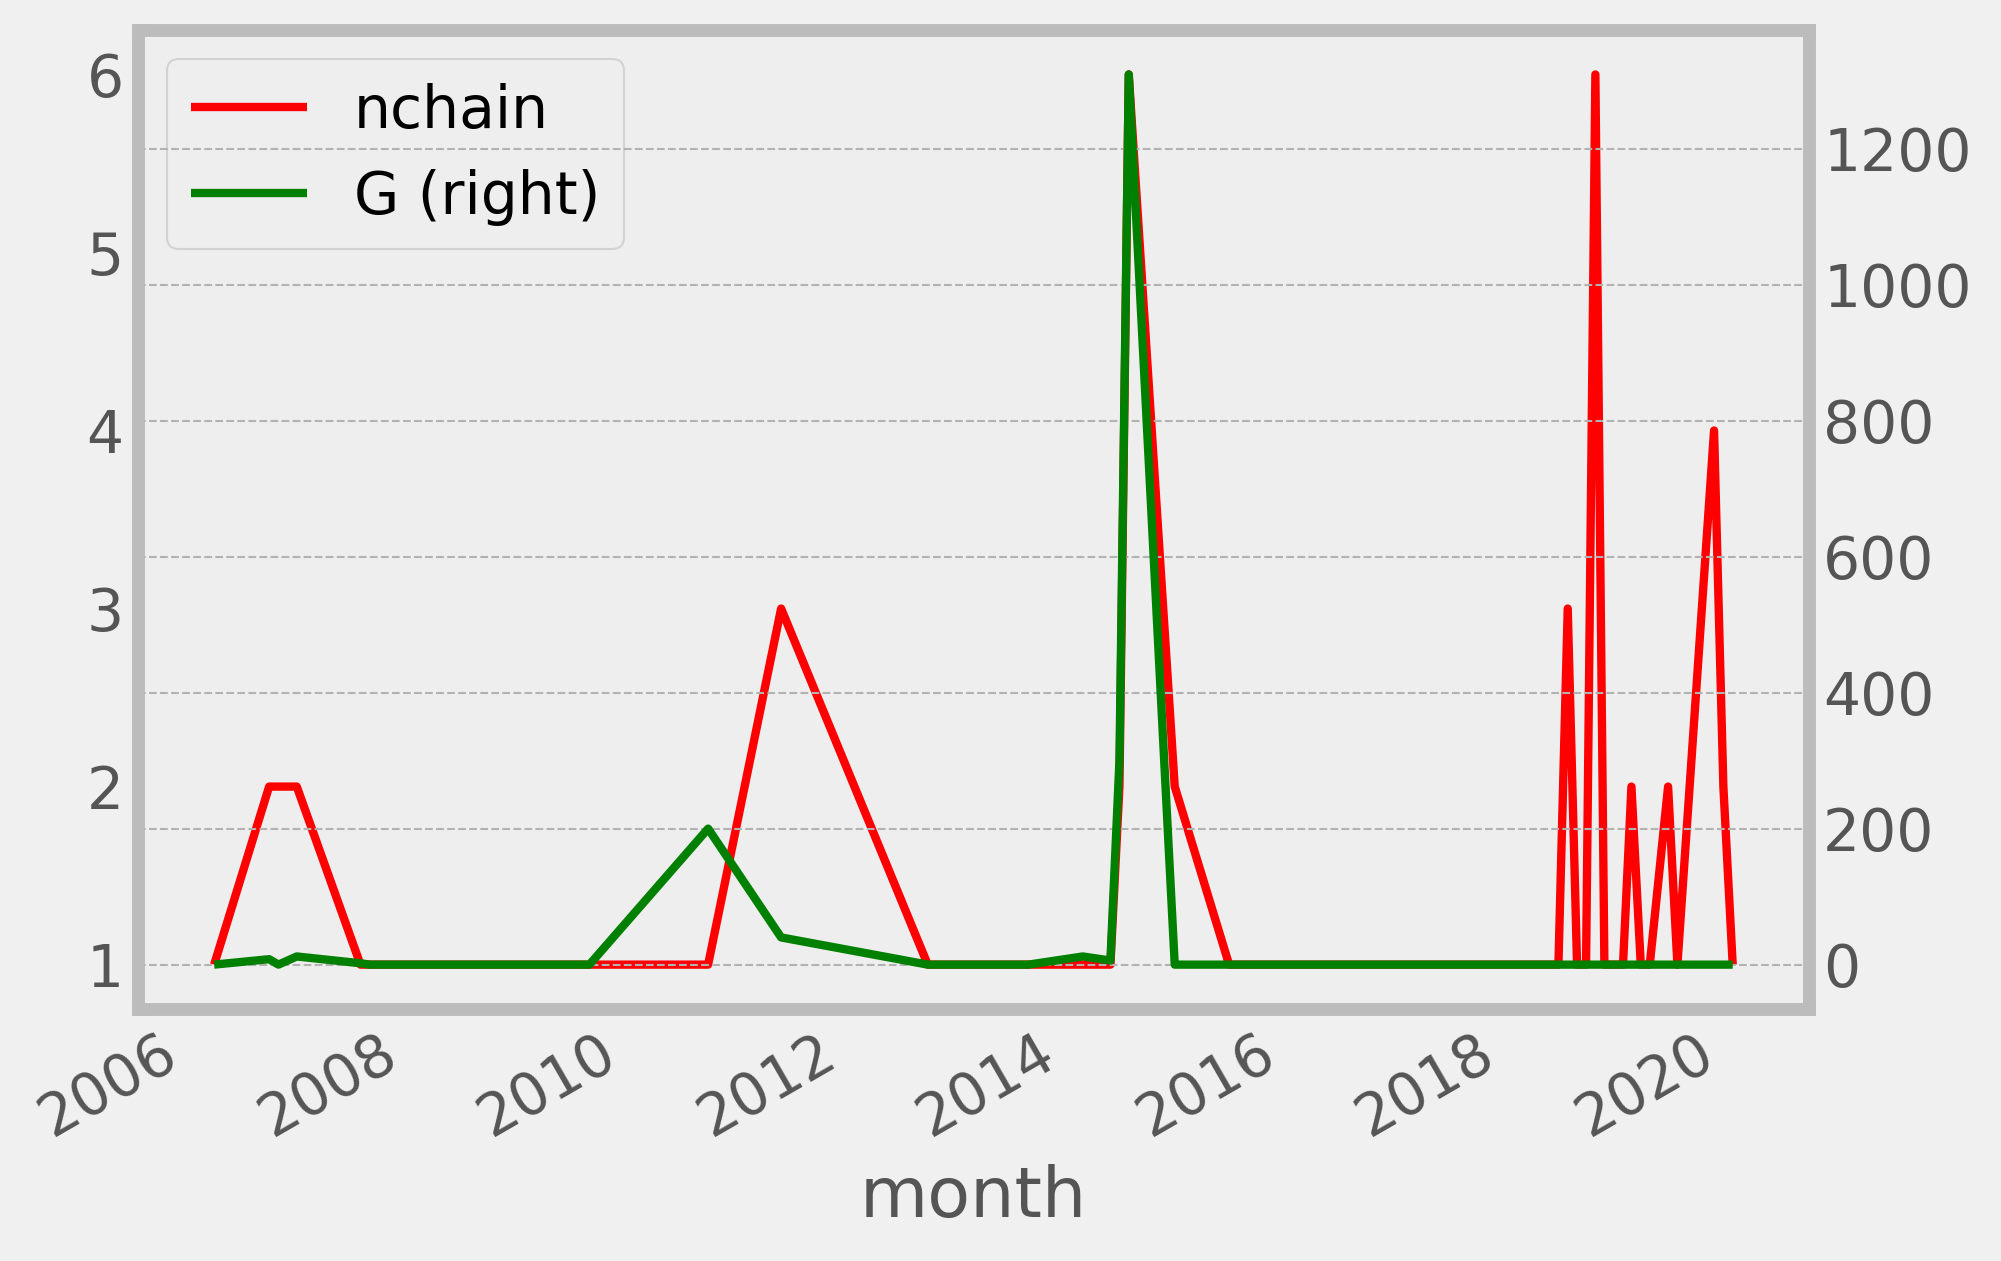
\includegraphics[width=0.7\textwidth]{./chapters/04/assets/chains_page.png}
    \caption{G and the number of chains for Barcelona page in Catalan.}
    \label{fig:chainsuser}
\end{figure}

\subsection{User}
\paragraph*{wars}
Table \ref{table:mean} ranks the users by the mean length of the chains they joined. All of them are anonymous users.
The longest chains are usually about details (like, for example, the number of championships won by Juventus) that are
continuously modified until the vandal is blocked.

\begin{table}[H]
    \centering
    \ra{1.2}
    \begin{tabularx}{\columnwidth}{@{}Xllll@{}}
        \midrule
        \textbf{id}& \textbf{user} & \textbf{nchains} & \textbf{mean}& \textbf{nrevert}  \\ \toprule
        1 & 95.20.240.x & 7  & 60.4 & 423 \\
        2 & 95.20.242.x & 1  & 51.0 & 51  \\
        3 & 37.11.145.x & 14  & 51.0 & 714  \\
        4 & 95.20.249.x & 14  & 51.0 & 714  \\
        5 & 83.49.253.x & 1  & 47.0 & 47 \\
        
         \bottomrule
    \end{tabularx}
    
    \caption{User sorted by mean length of the chains joined \label{table:mean}}
\end{table}

It is also possible to see on which pages a given user joins more revert wars. Table
\ref{table:pagesuser}  represents the pages on which the user, let us call him Juan, got involved in more chains in The Catalan
Wikipedia. In this example, Juan is mainly interested in Catalan famous people
like sportsmen and writers.

\begin{table}[H]
    \centering
    \ra{1.2}
    \begin{tabularx}{\columnwidth}{@{}Xllll@{}}
        \midrule
        \textbf{id}& \textbf{user} & \textbf{nchains}  \\ \toprule
        1 & Marc Márquez i Alentà & 14  \\
        2 & Barcelona & 9   \\
        3 & Jocs Olímpics d'estiu de 1992 & 7   \\
        4 & Rafael Nadal i Parera & 6  \\
        5 & Catalunya &  6 \\
        6 & Lliga de Campions de la UEFA	 &  6 \\
        7 & Quim Monzó &  6 \\
        8 & Polseres vermelles &  6 \\
        9 & Jordi Sànchez i Zaragoza &  6 \\
        10 & Alfons Arús i Leita &  6\\

         \bottomrule
    \end{tabularx}
    
    \caption{Top 10 pages by number of chain of Juan. \label{table:pagesuser}}
\end{table}
\paragraph*{monthly}
Given a user we can draw its revert chain activity. 
\begin{figure}[H]
    \centering
    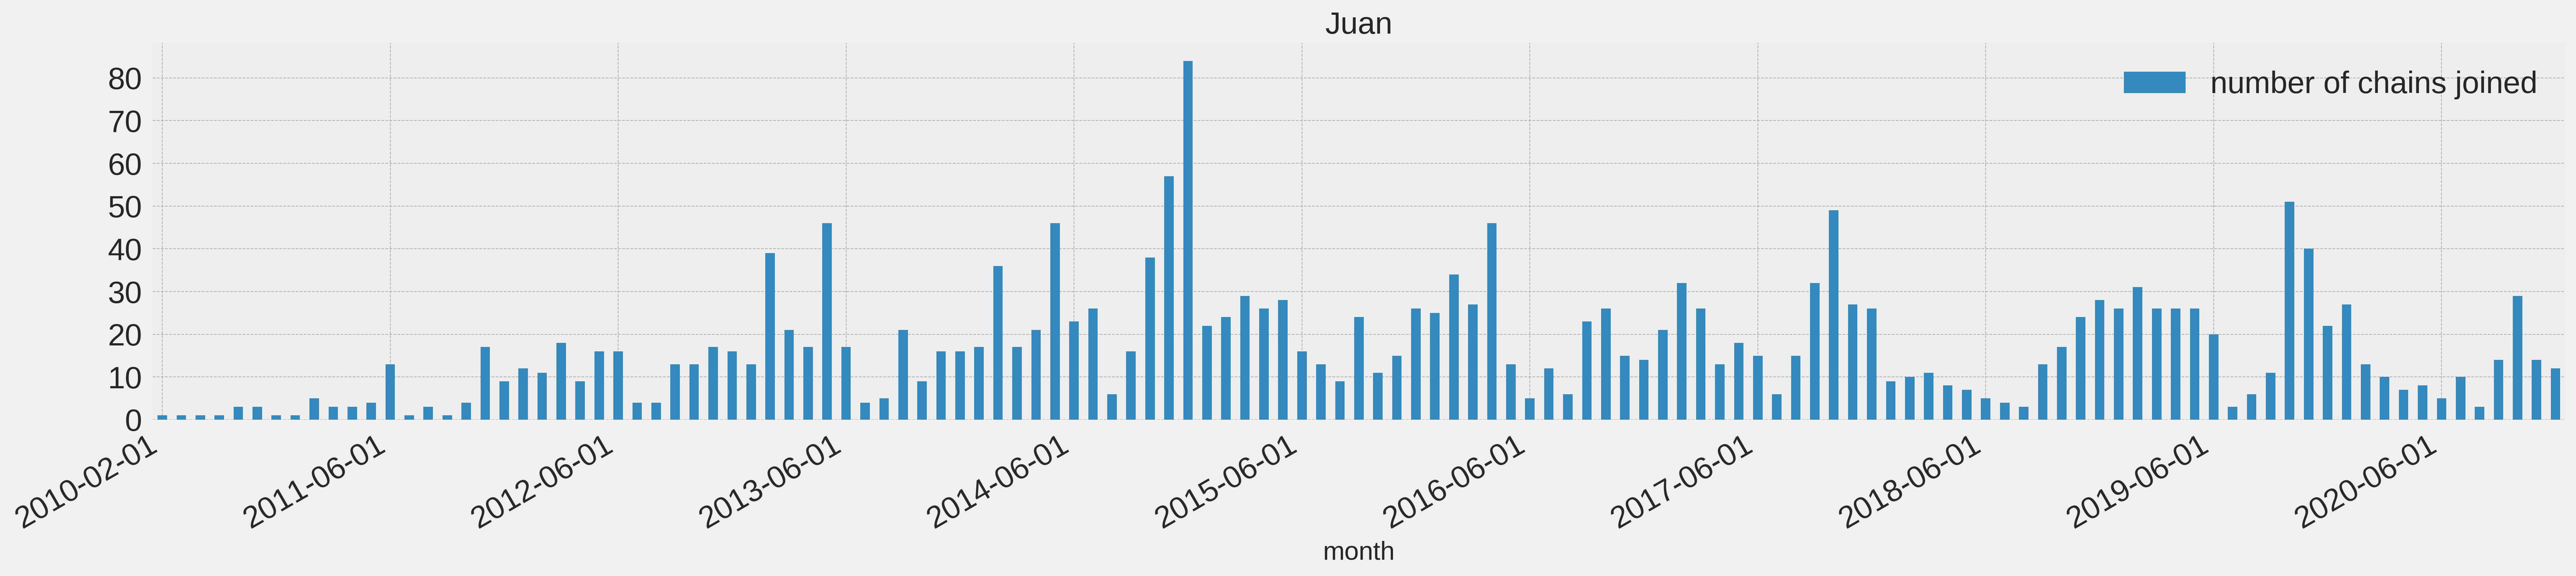
\includegraphics[width=\textwidth]{./chapters/04/assets/chains_user_month.png}
    \caption{Number of chain by month of Juan}
    \label{fig:chainsusermonth}
\end{figure}

\section{Group}
From the analysis of the groups, we can define different rankings of pages using the number of
reverts of each group. Given a page, we can plot the trend of the edits by group and detect the
pages in which the admins are more interested. We can say from which category a given user
is the target of reverts and the ratio between made and received reverts. Such a deep analysis of
this data can be done, that is the reason why it is available to everyone who needs it. 

Here are some numbers about the users in different languages:
\begin{table}[H]
    \centering
    \ra{1.2}
    \begin{tabularx}{\columnwidth}{@{}Xrrr@{}}
        \midrule
        \textbf{len}& \textbf{registered} & \textbf{admin}& \textbf{active}  \\ \toprule
        en& 41,825,139& 1,089& 127,566  \\
        es & 6'266'812 & 69 & 16'143   \\
        it & 2'140'498 & 114 & 8'208\\
        ca & 391'067 & 22 & 1'180   \\
     


         \bottomrule
    \end{tabularx}
    
    \caption{Number of users by group. \label{table:statsuser}}
\end{table}

\subsection{Page}
\paragraph*{reverts}
In Fig \ref{fig:compare} we can see how the influence of the admins is higher in the Italian
Wikipedia than in the Spanish one. All the spikes we can see in Spanish and Catalan Wikipedias are due to the
seasonality of the user activity: every year during the summer there is a decrease in the edits and
therefore of the reverts. In Catalan, these trends are more visible, and we can see that the number of
reverts made by admin towards registered users is similar to the ones done by registered toward
registered unlike the Italian and Spanish ones. 
\begin{figure}[H]
    \centering
    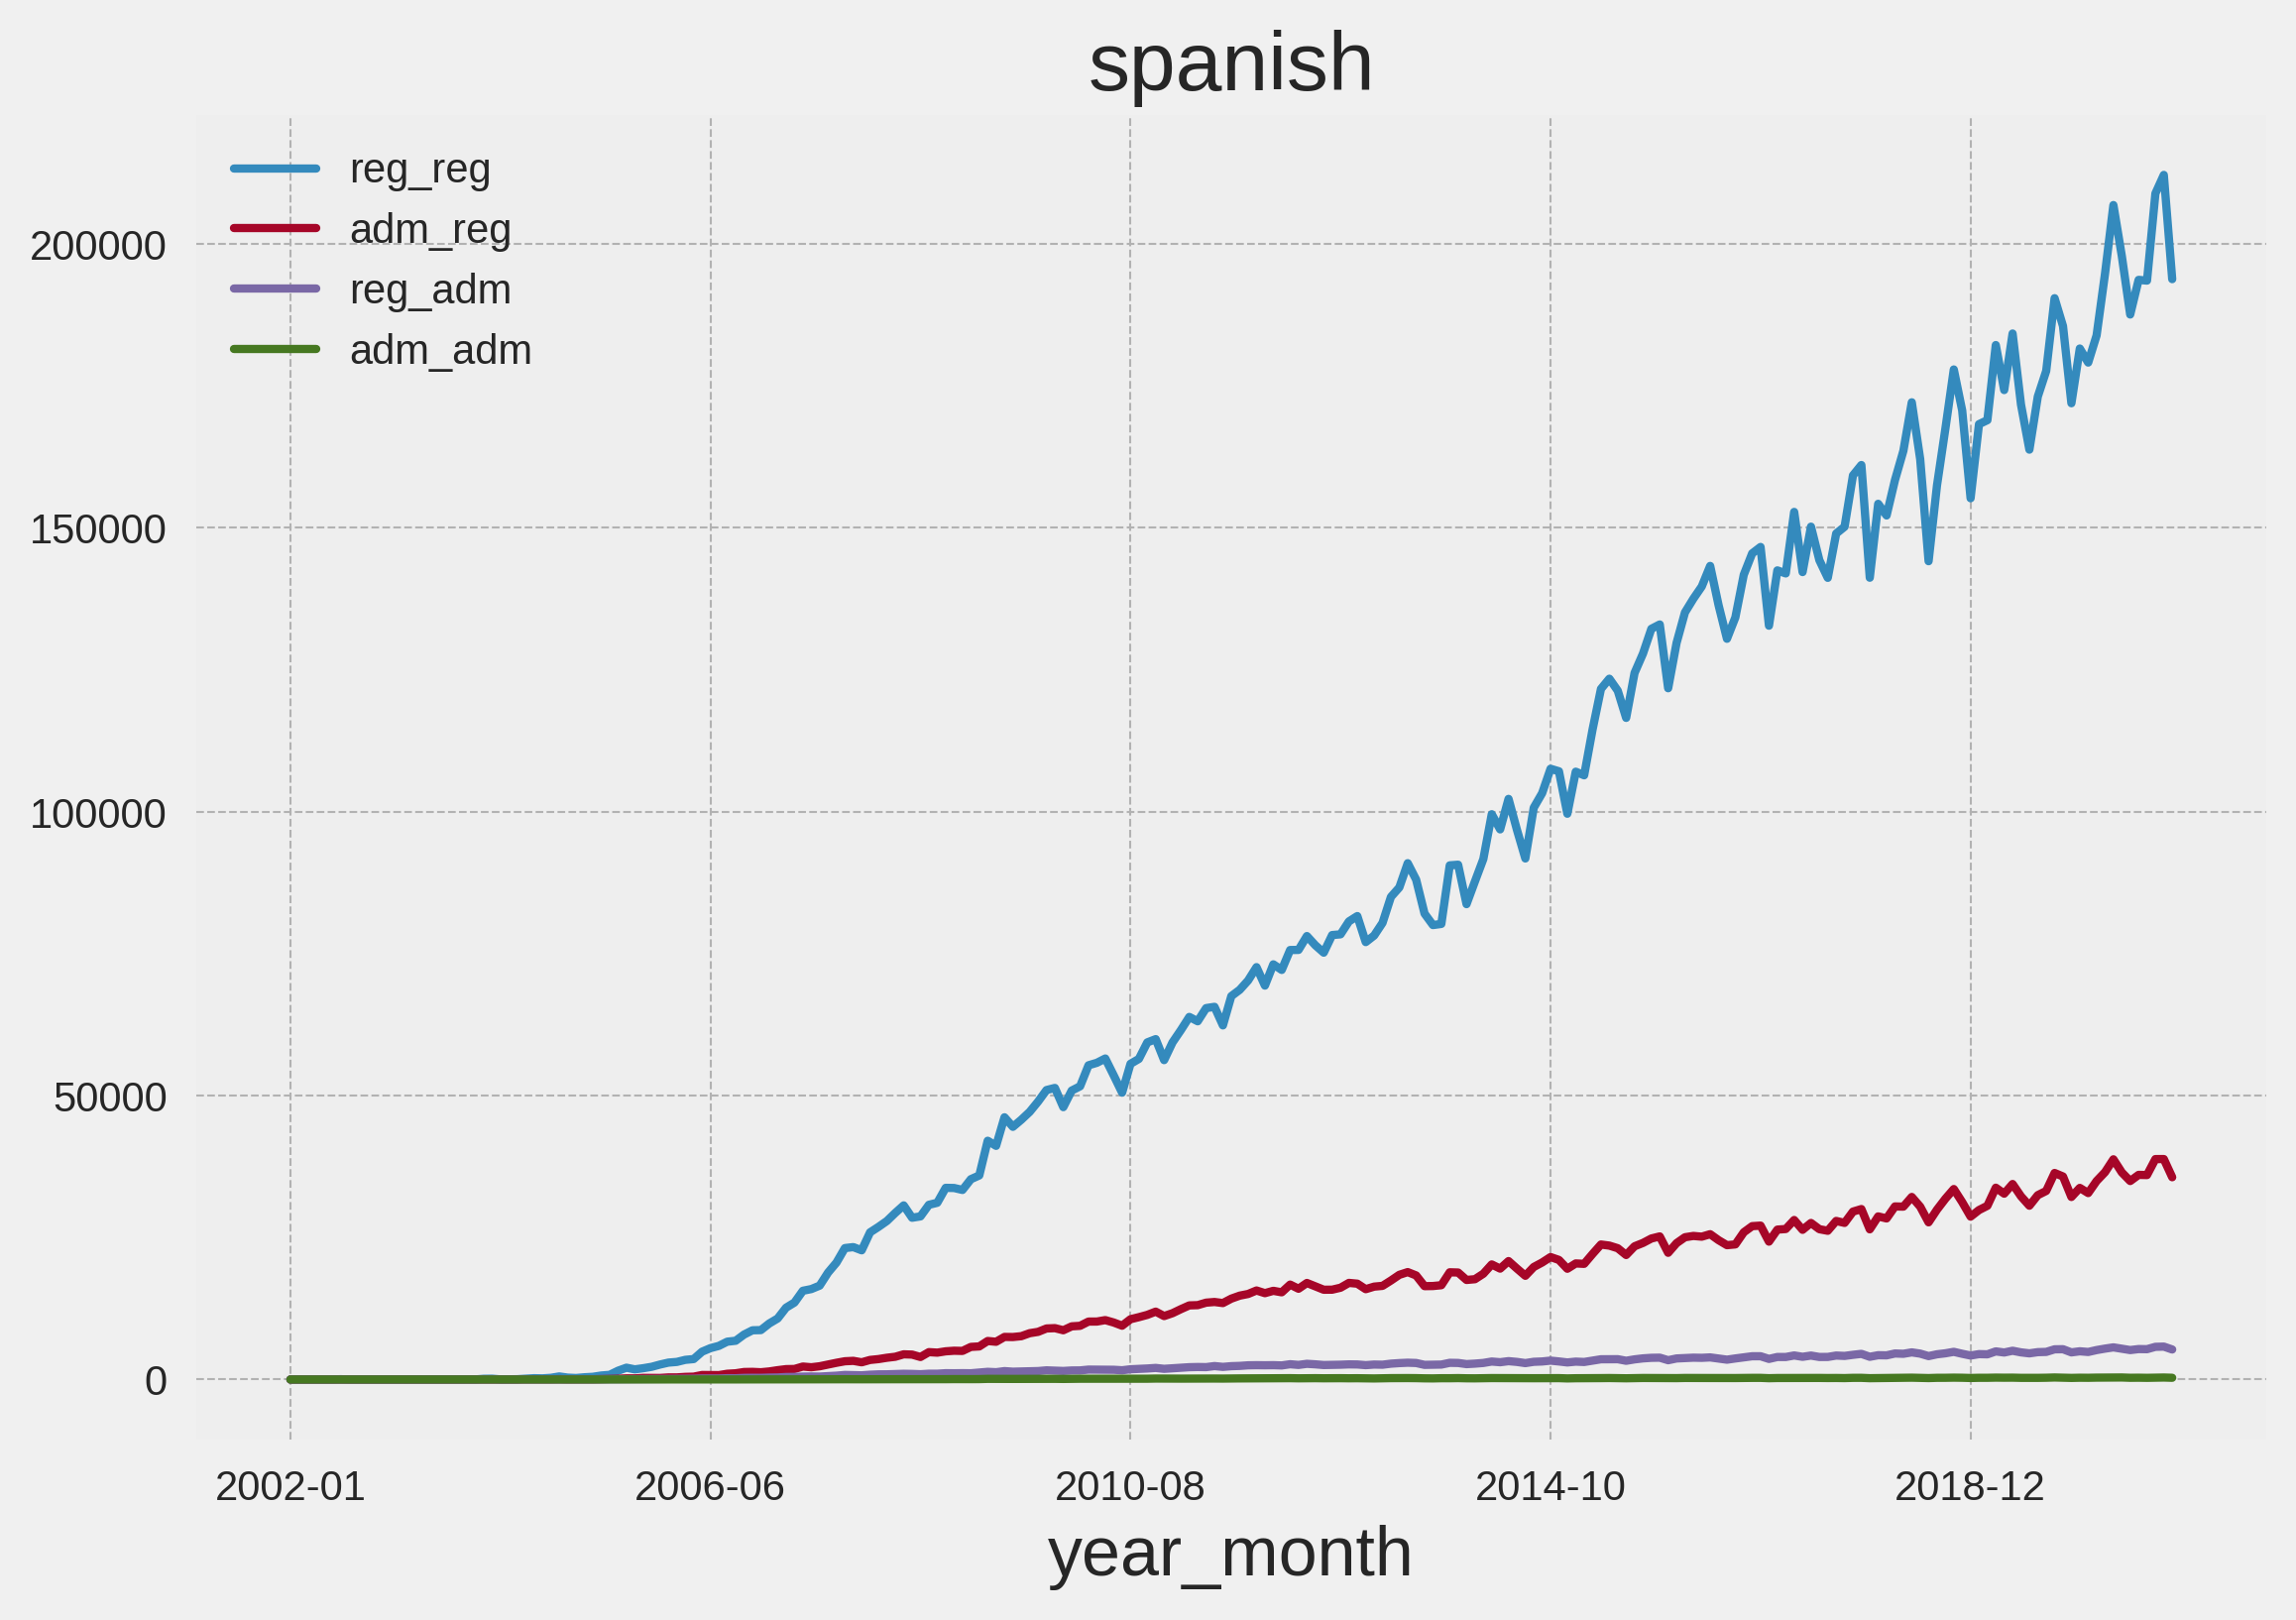
\includegraphics[width=0.45\textwidth]{./chapters/04/assets/admin_es.png}
    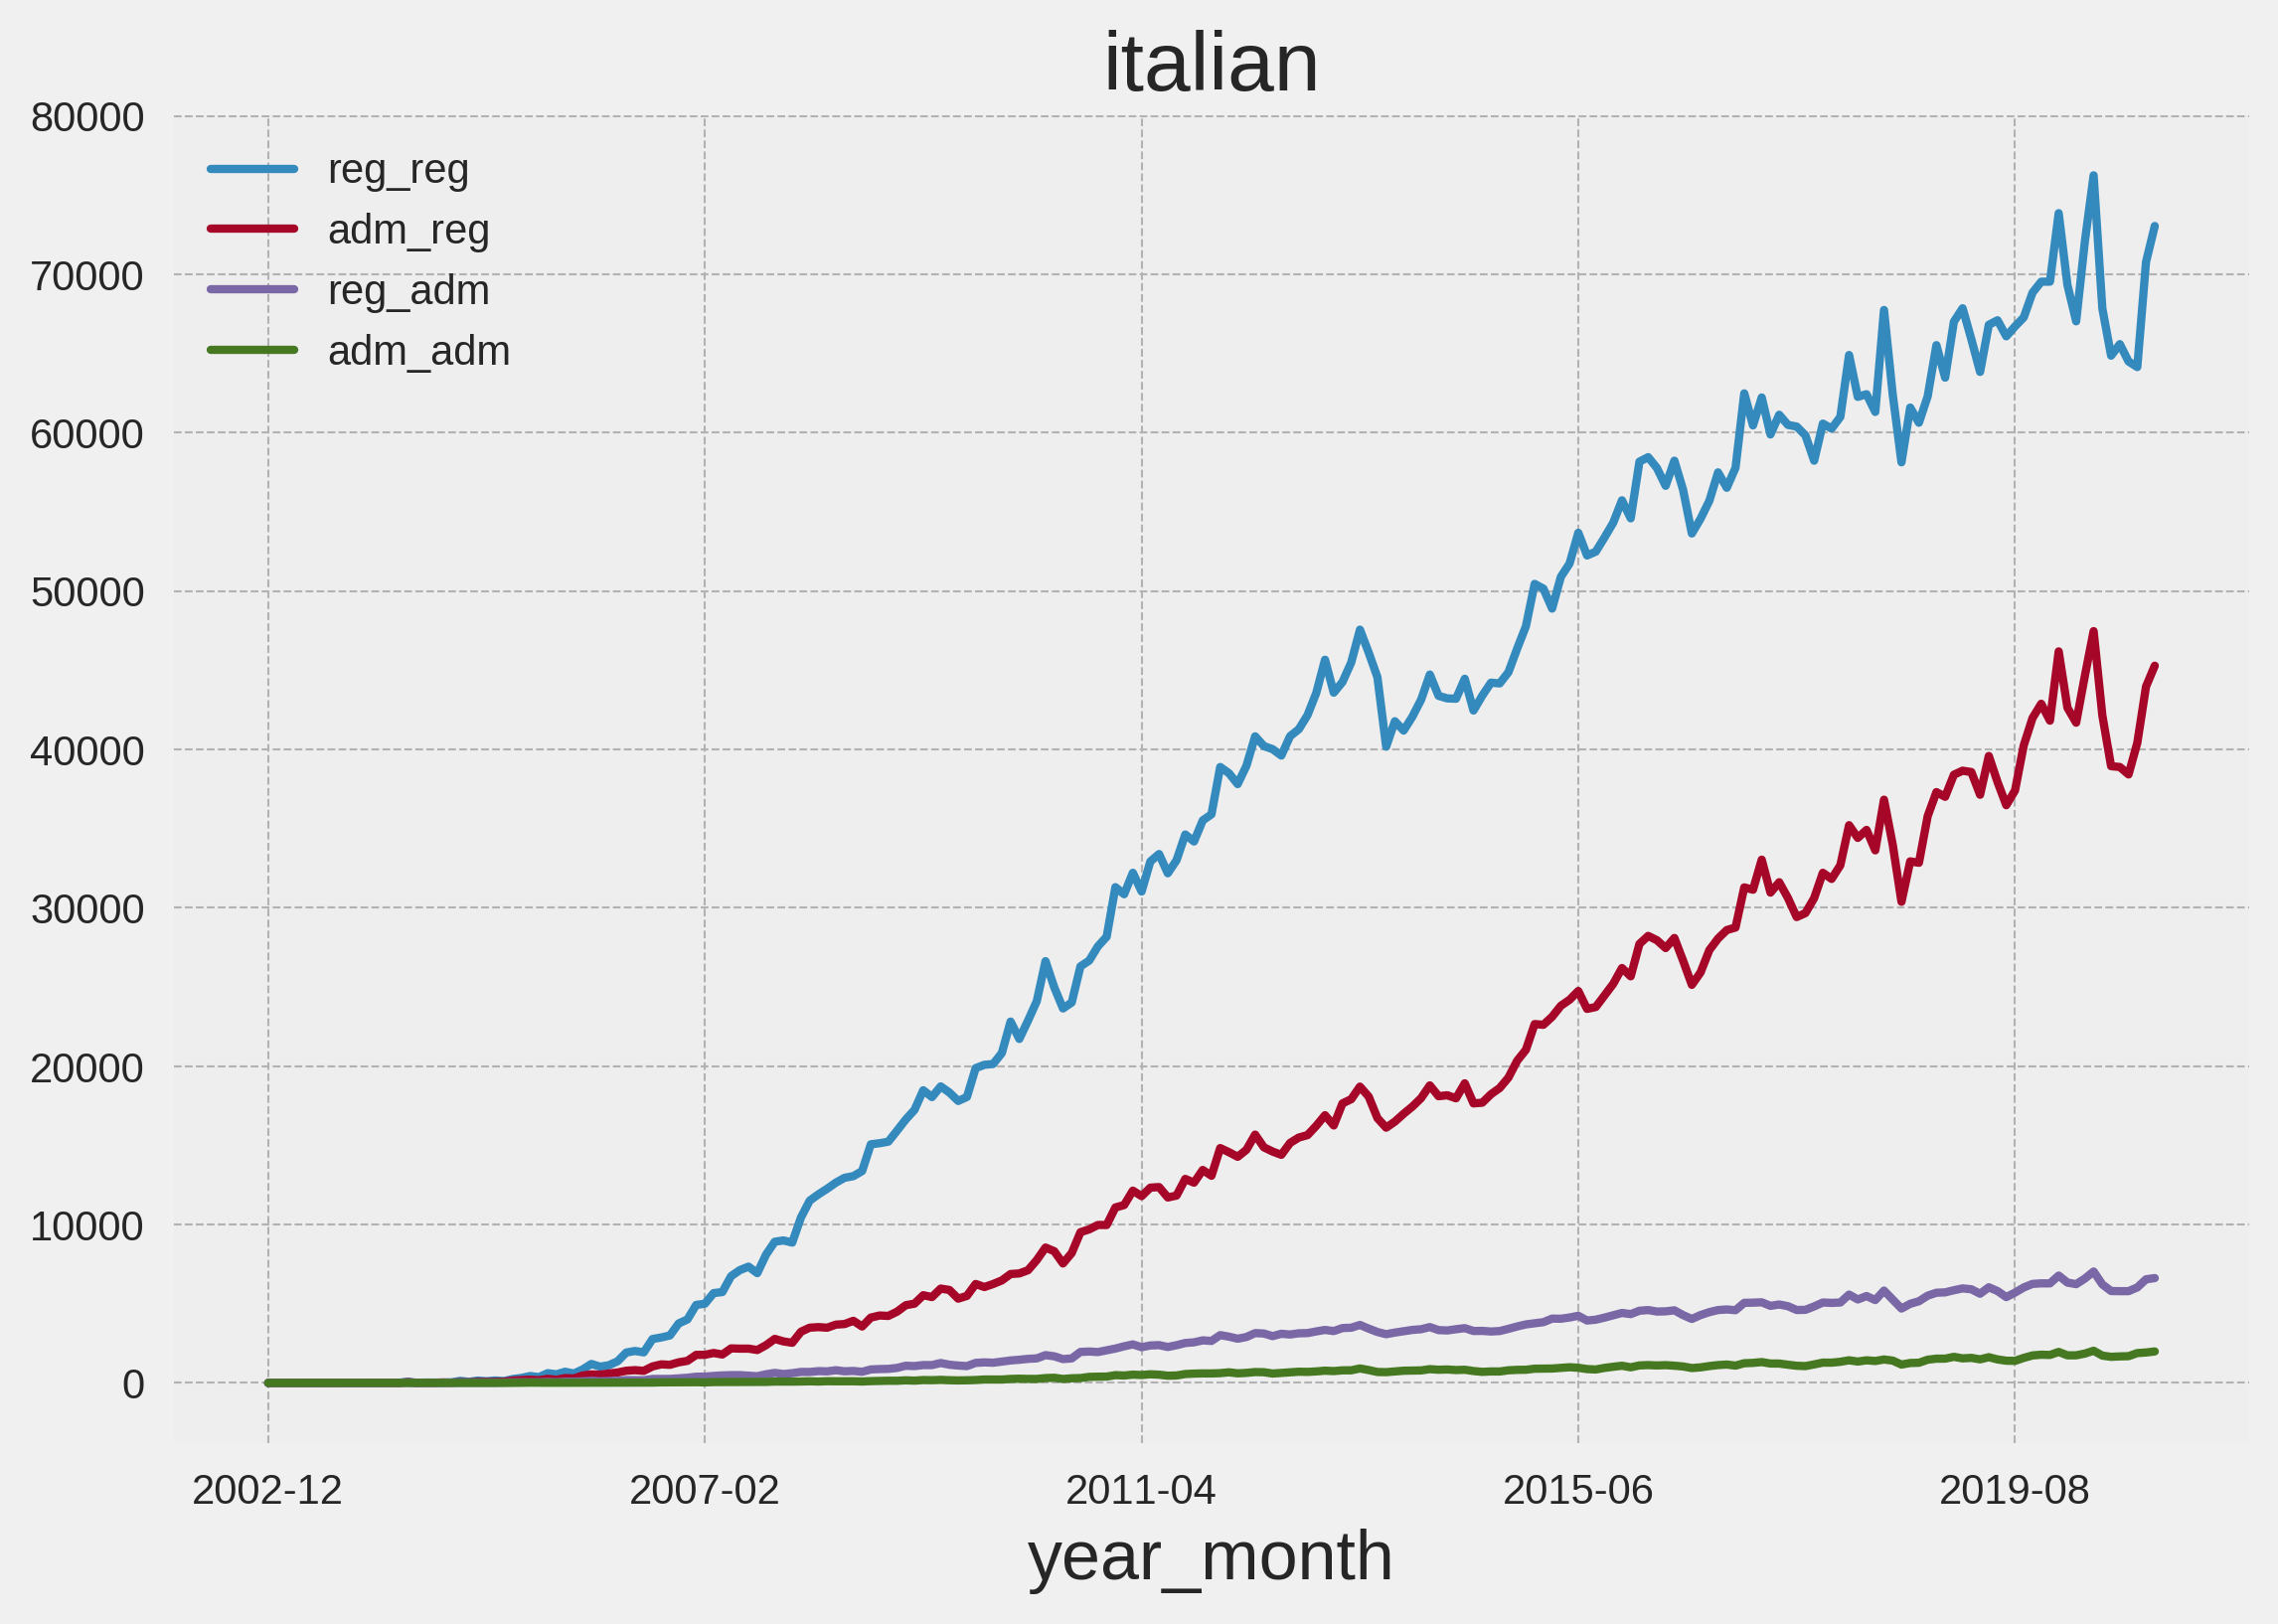
\includegraphics[width=0.45\textwidth]{./chapters/04/assets/admin_it.png}
    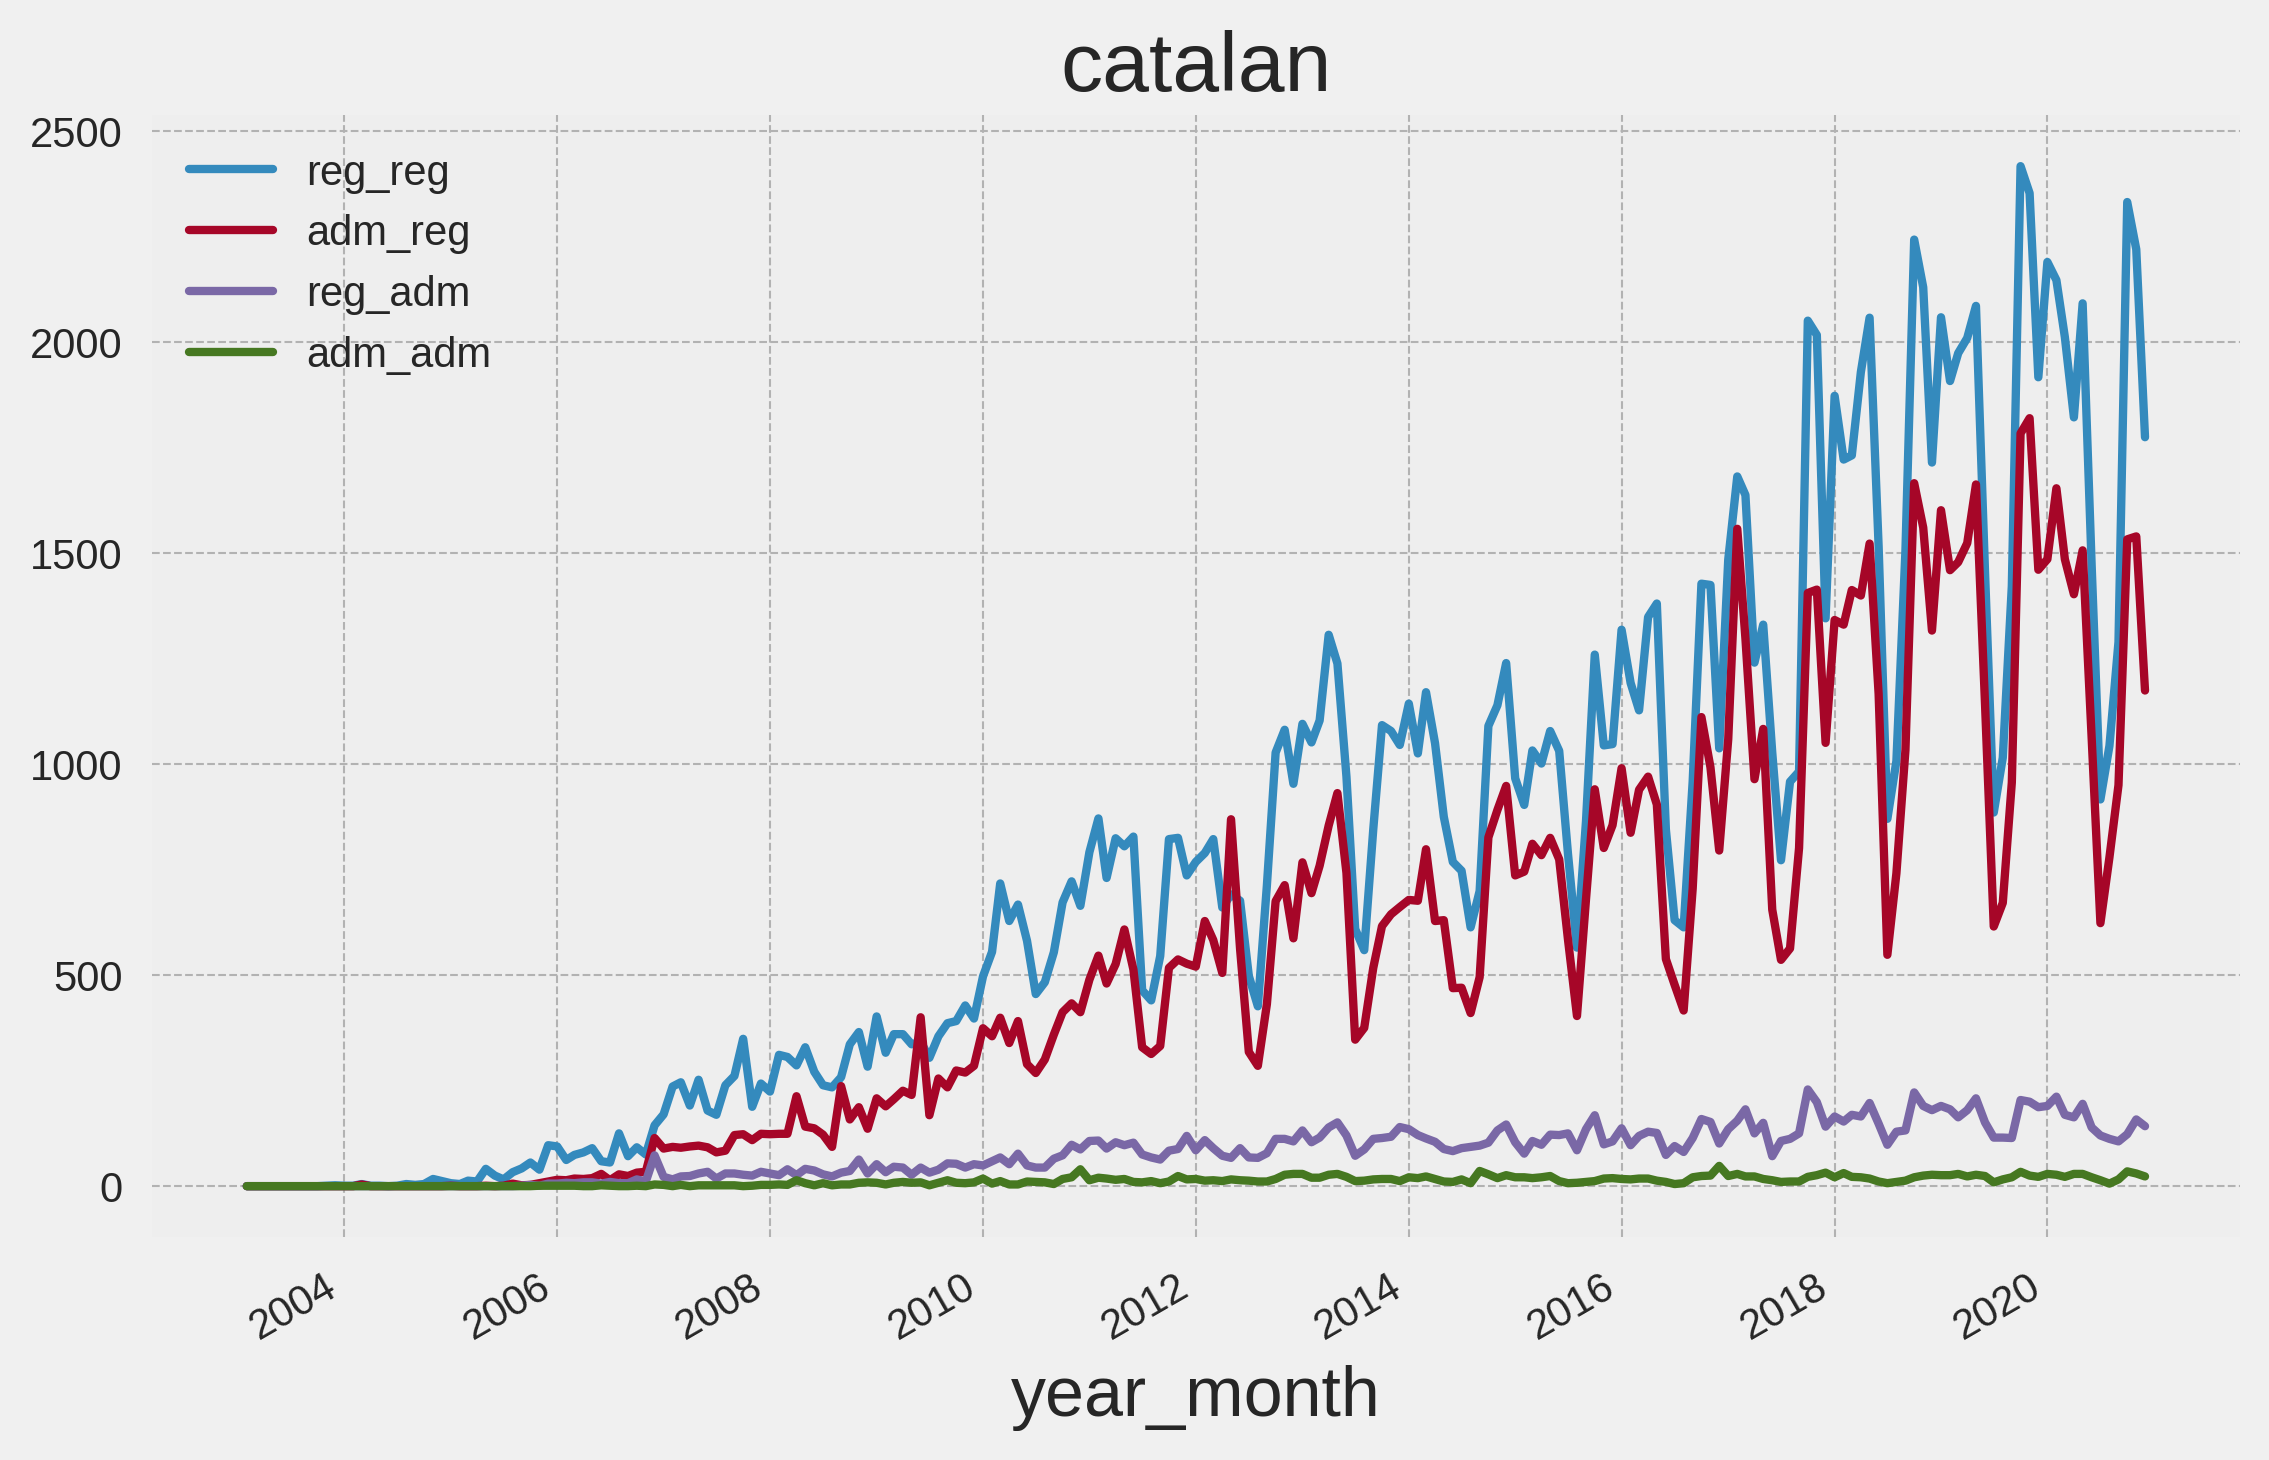
\includegraphics[width=0.45\textwidth]{./chapters/04/assets/admin_ca.png}
    \caption{Number of reverts done divided by group.}
    \label{fig:compare}
\end{figure}
\paragraph*{mutual}
In this graph, we can see a comparison between M and the total number of reverts done and we can
notice that M had a big growth until 2019 where it remained stable.
\begin{figure}[H]
    \centering
    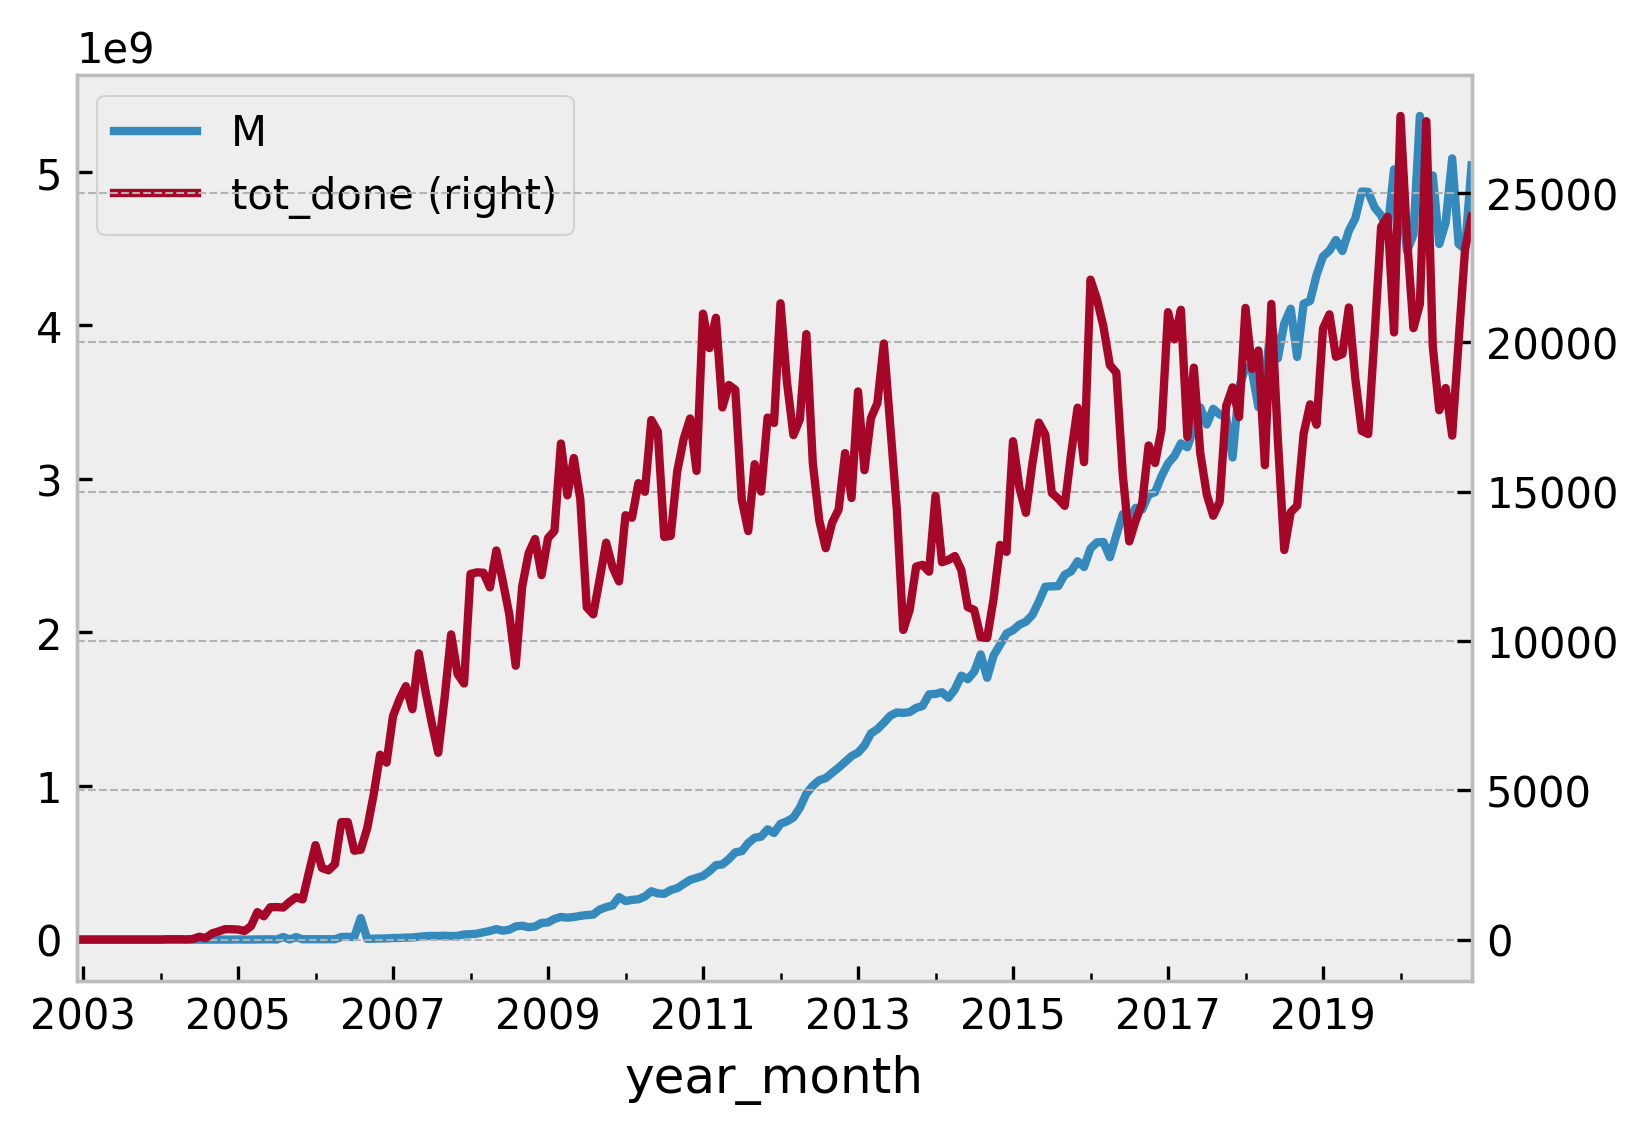
\includegraphics[width=0.6\textwidth]{./chapters/04/assets/Mcompare.png}
    \caption{mcompare}
    \label{fig:M compared to the number of Reverts}
\end{figure}
\subsection{User}
From the analysis of the reverts devided by group we are able to see the influence of admins and the
distribution of the revert done and received during the months. It is possible to know, for a given
user, how many reverts he received and made to each category.
\paragraph*{reverts}
The plots represent, for Italian, Catalan and Spanish, the number of reverts done and received by
each category; we can see how the behaviour of the users changes with the language especially
towards anonymous users. The Italian and the Spanish trends on done reverts are similar, but the share of
the reverts of the admin in the received ones is very different. In Italy, the received reverts are
equally divided between anonymous and registered.  
\begin{figure}[H]
    \centering
    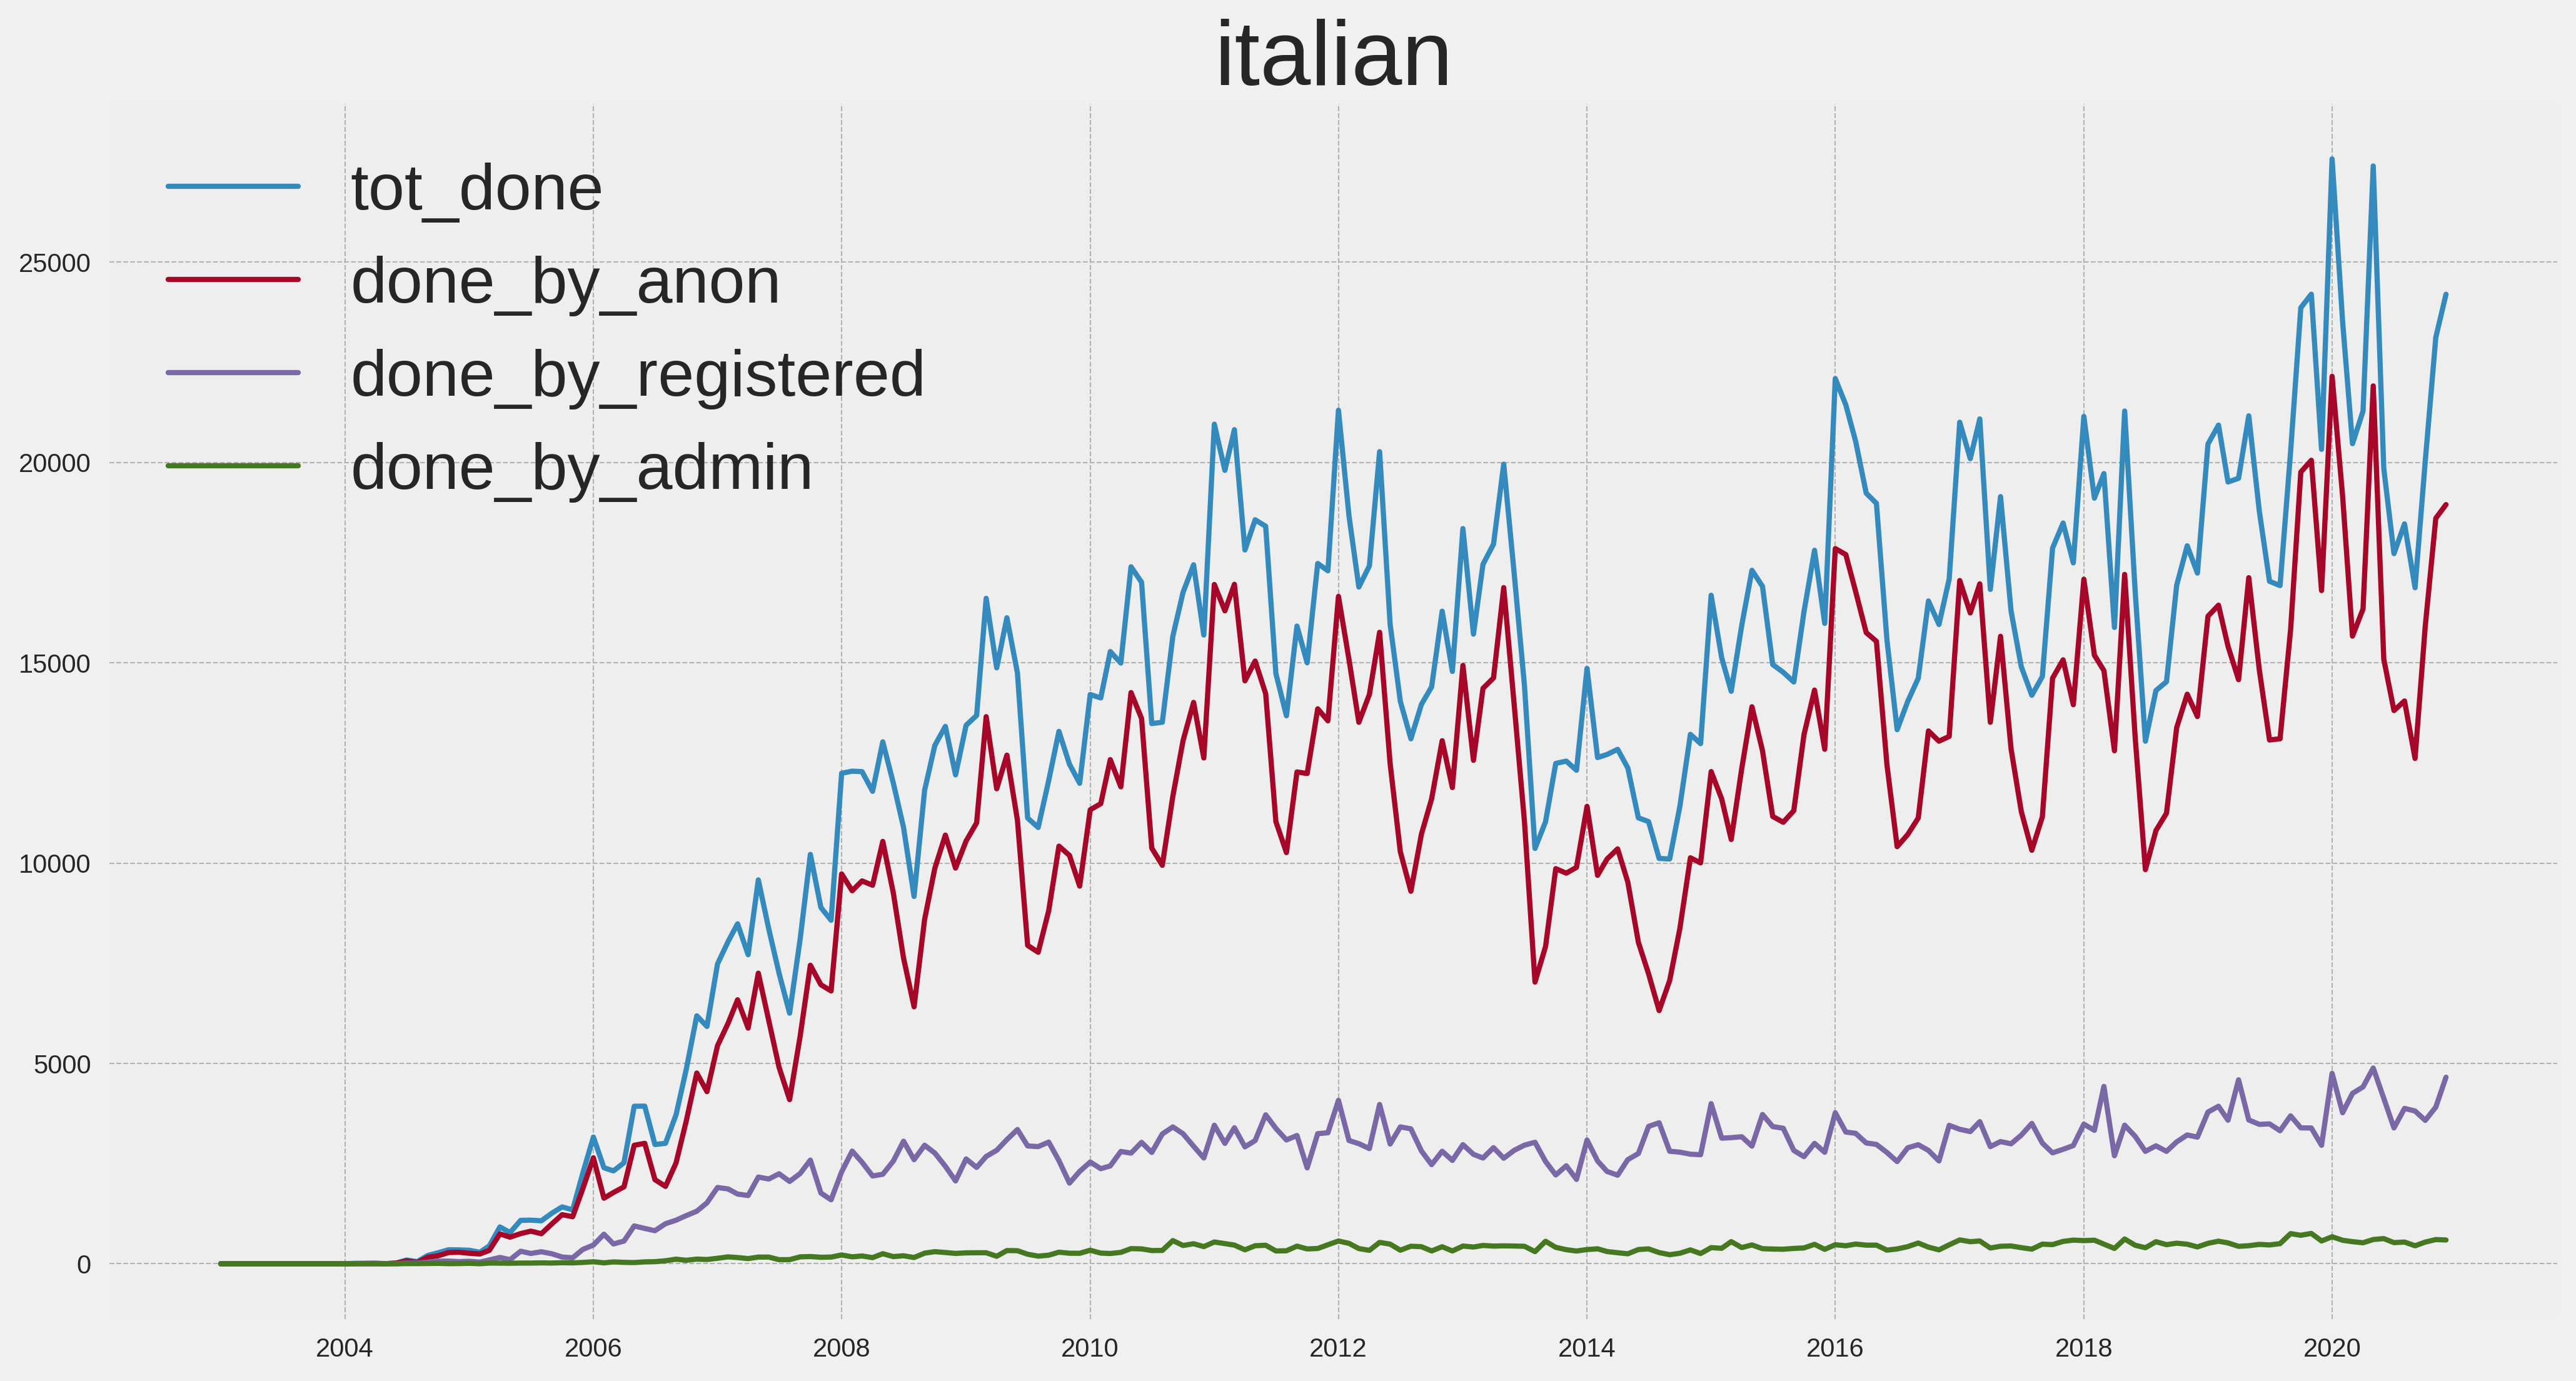
\includegraphics[width=0.49\textwidth]{./chapters/04/assets/revert_done_it.png}
    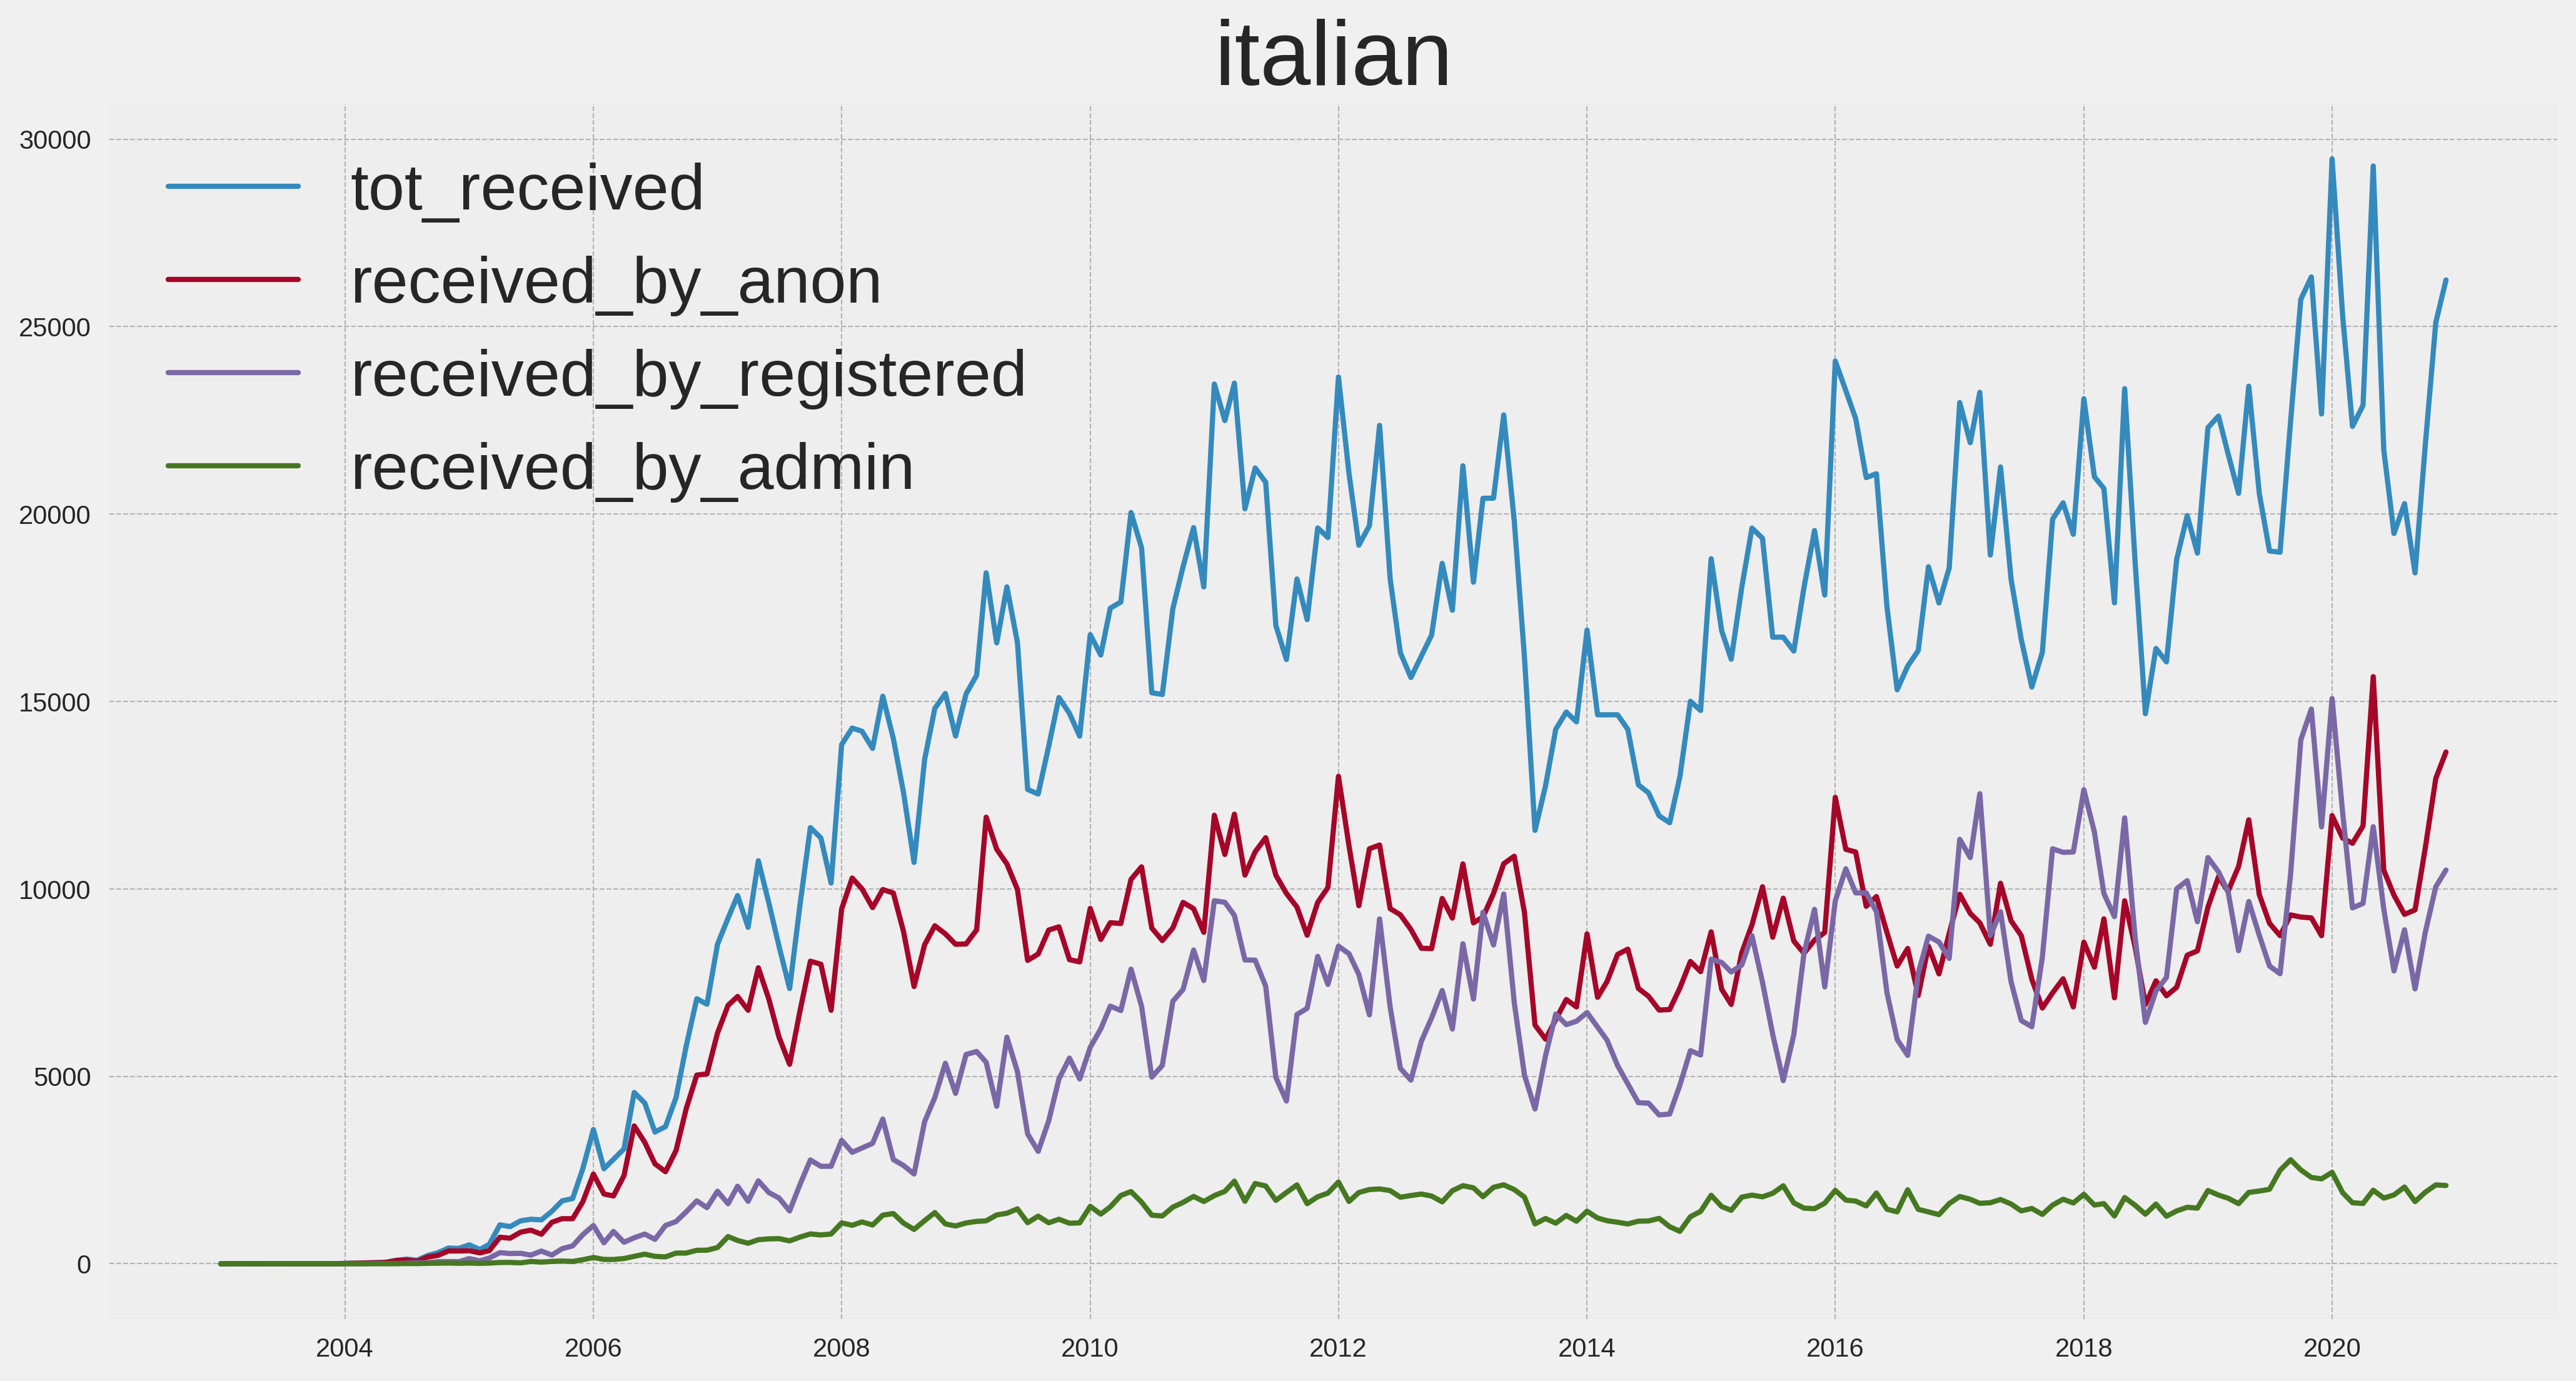
\includegraphics[width=0.49\textwidth]{./chapters/04/assets/revert_received_it.png}
    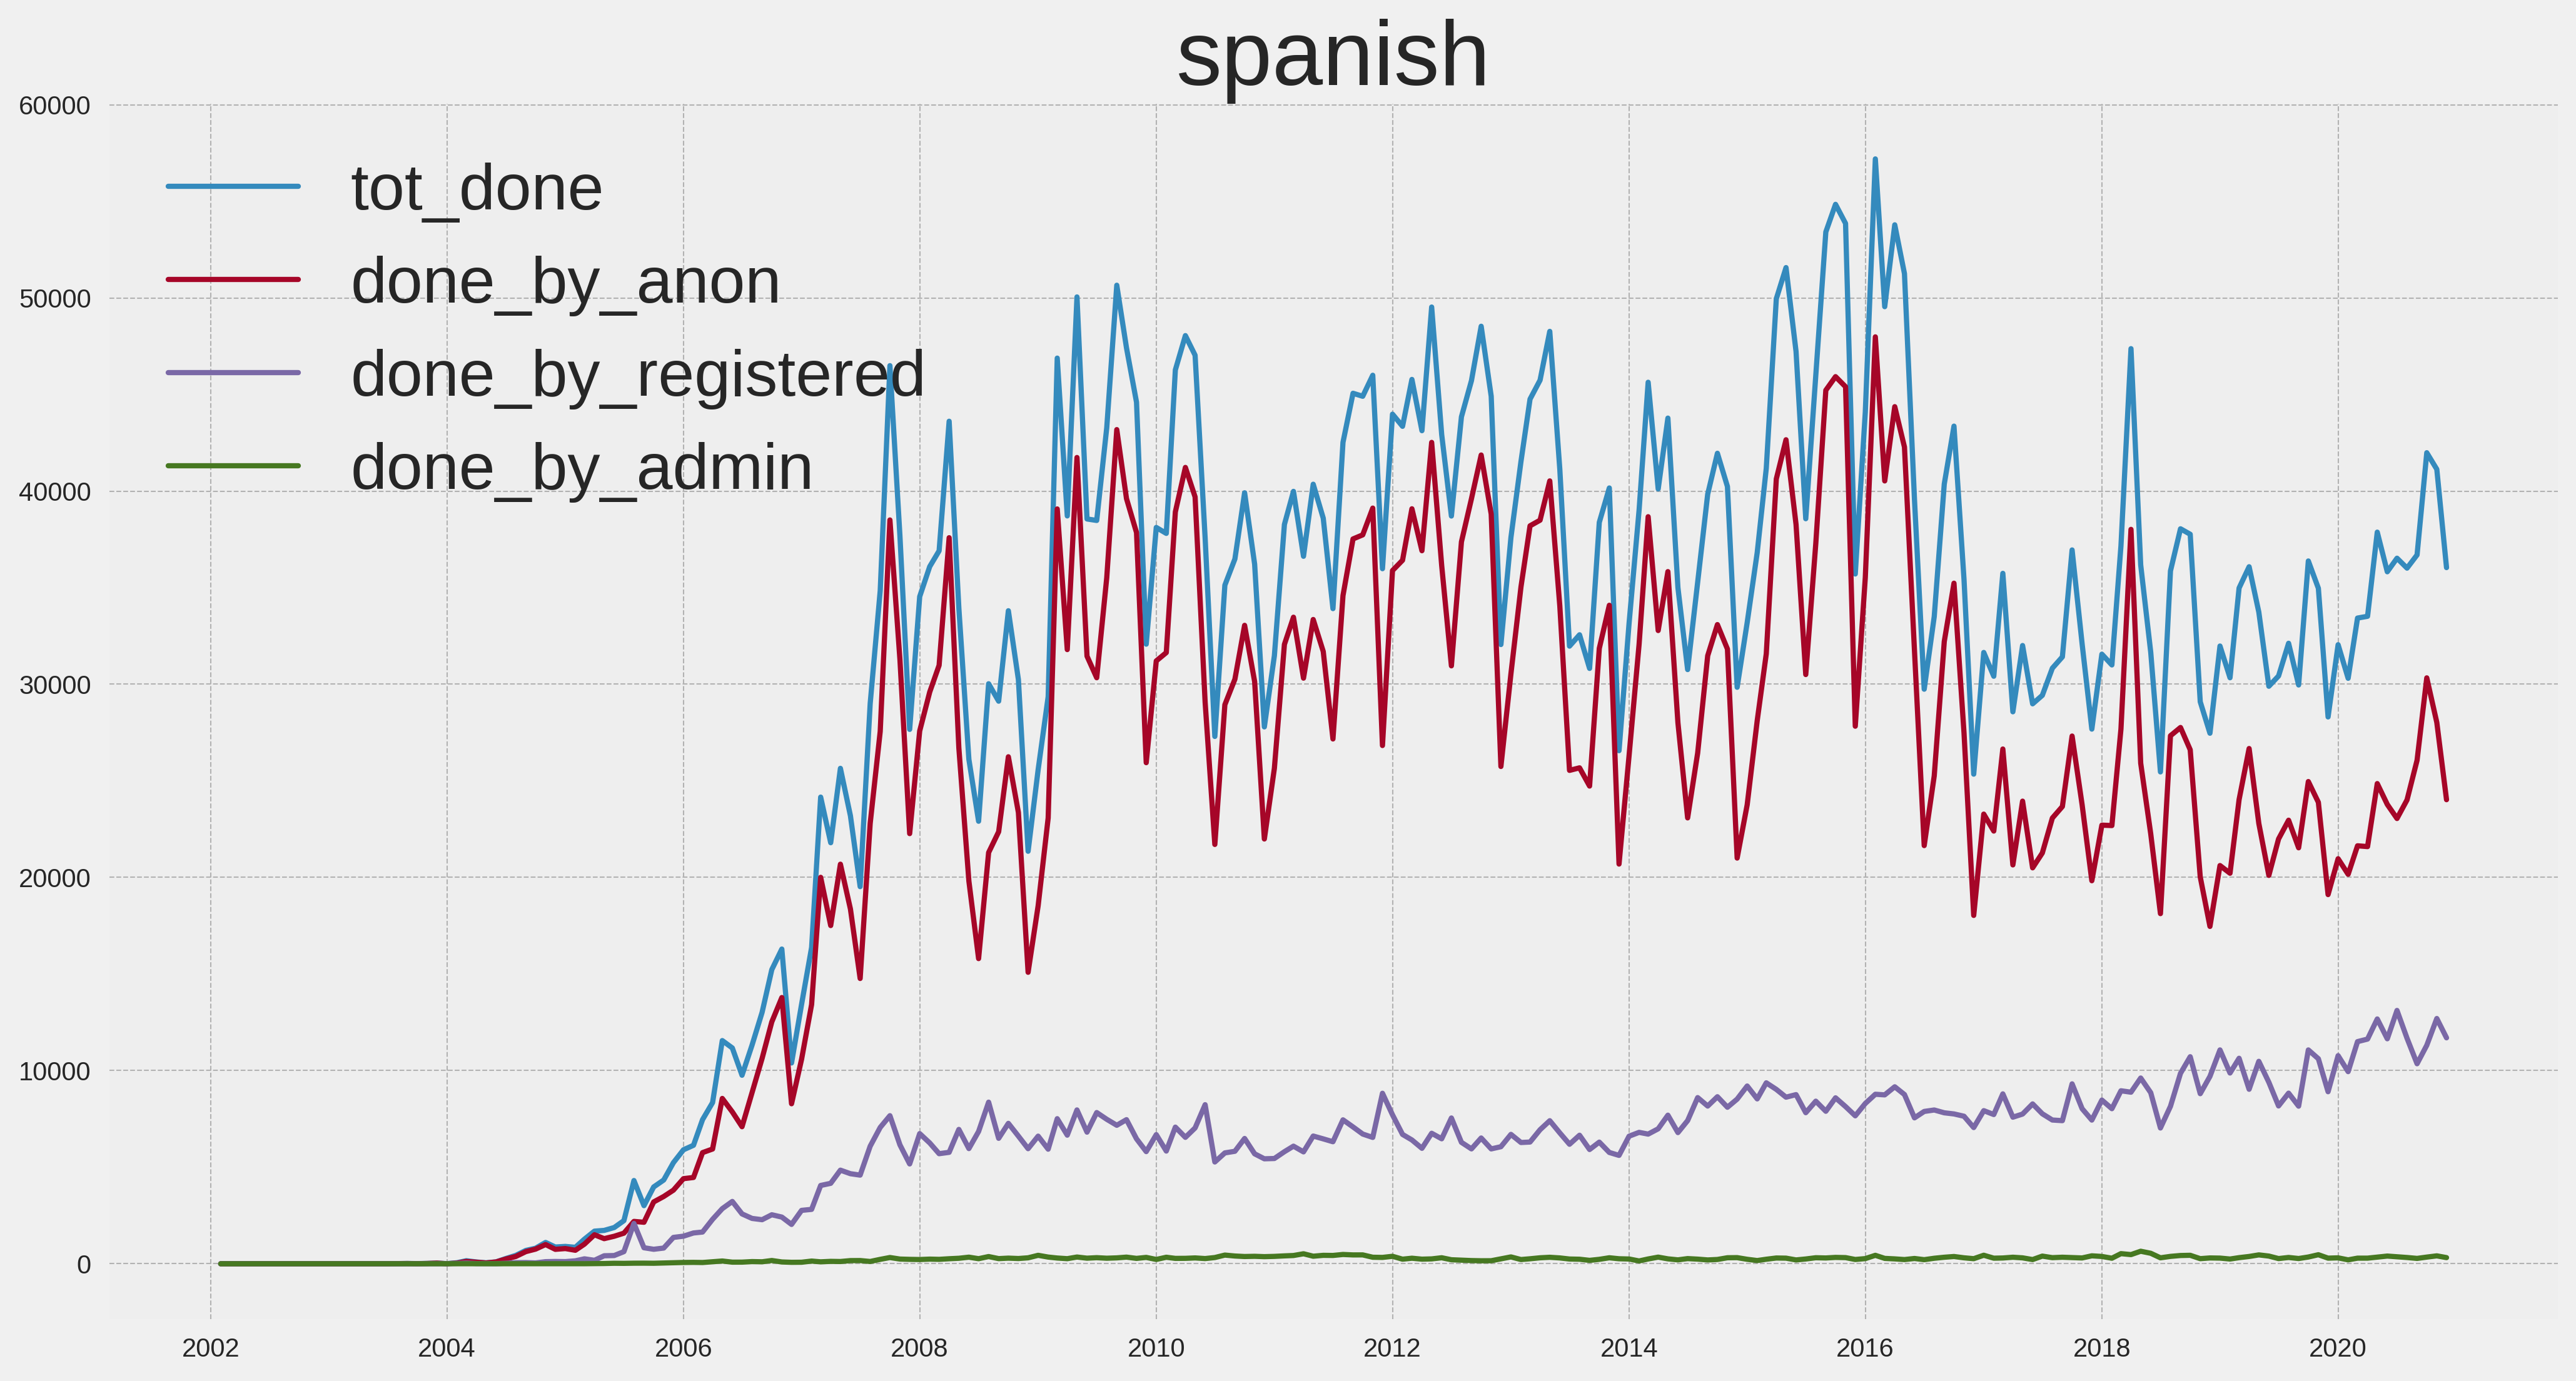
\includegraphics[width=0.49\textwidth]{./chapters/04/assets/revert_done_es.png}
    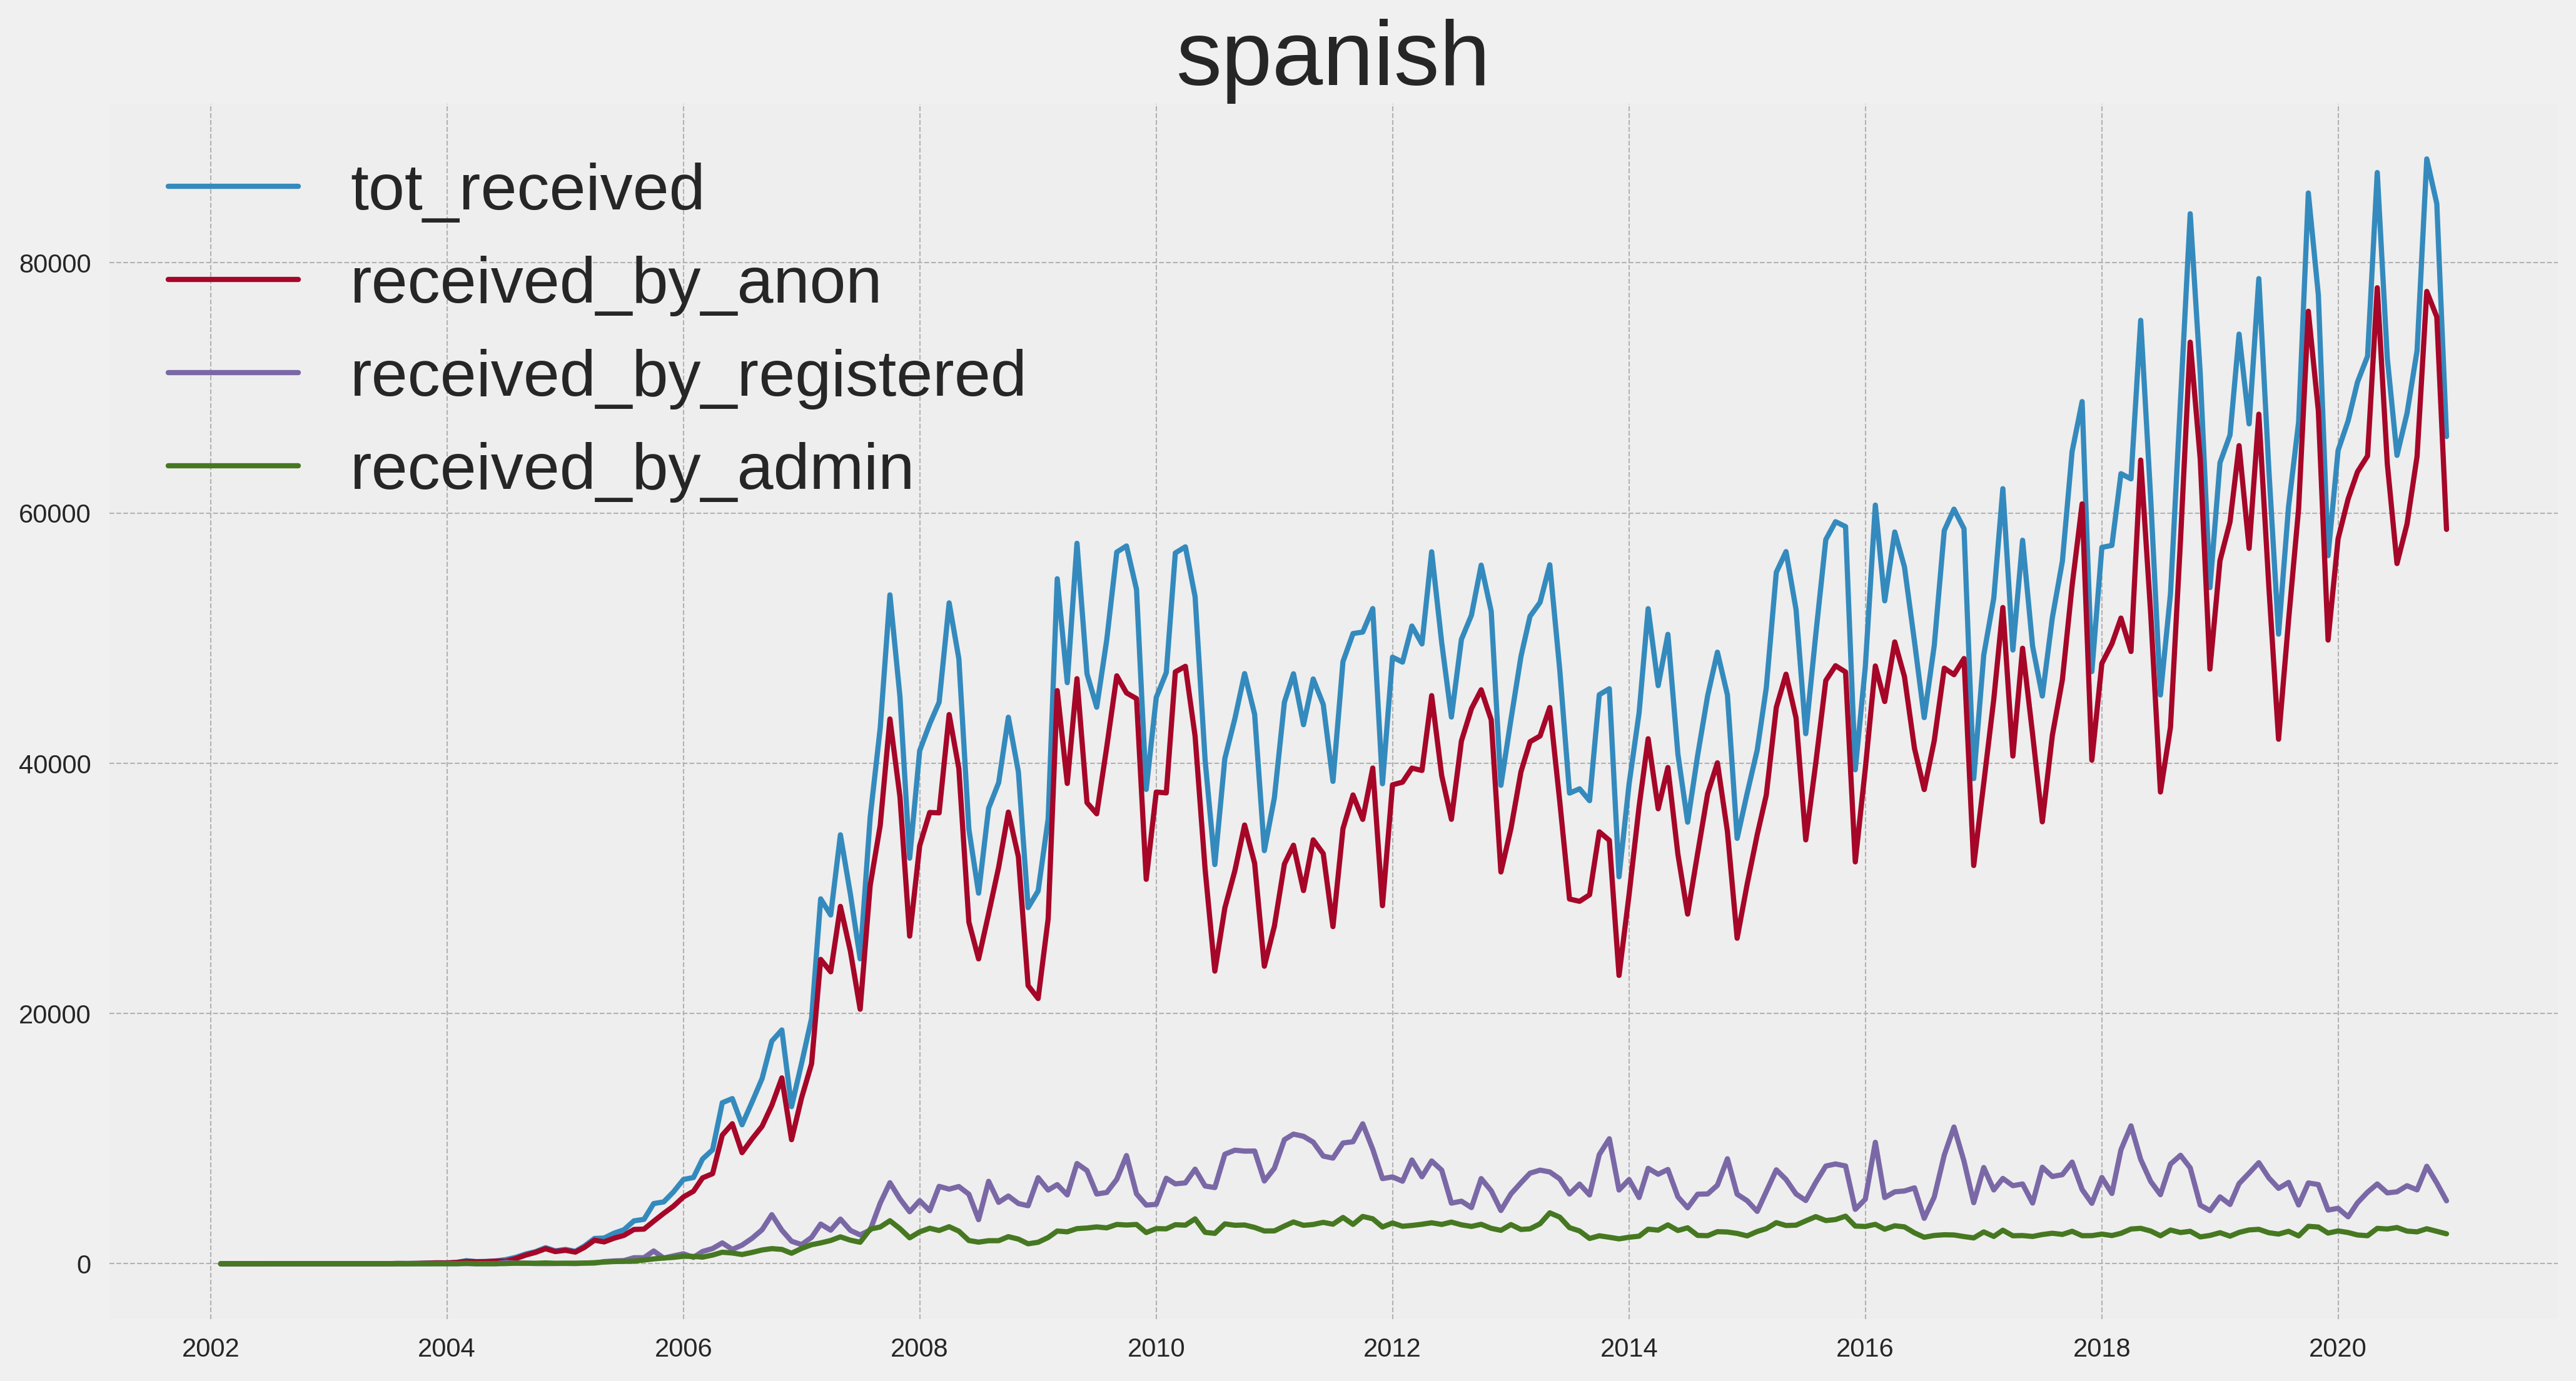
\includegraphics[width=0.49\textwidth]{./chapters/04/assets/revert_received_es.png}
    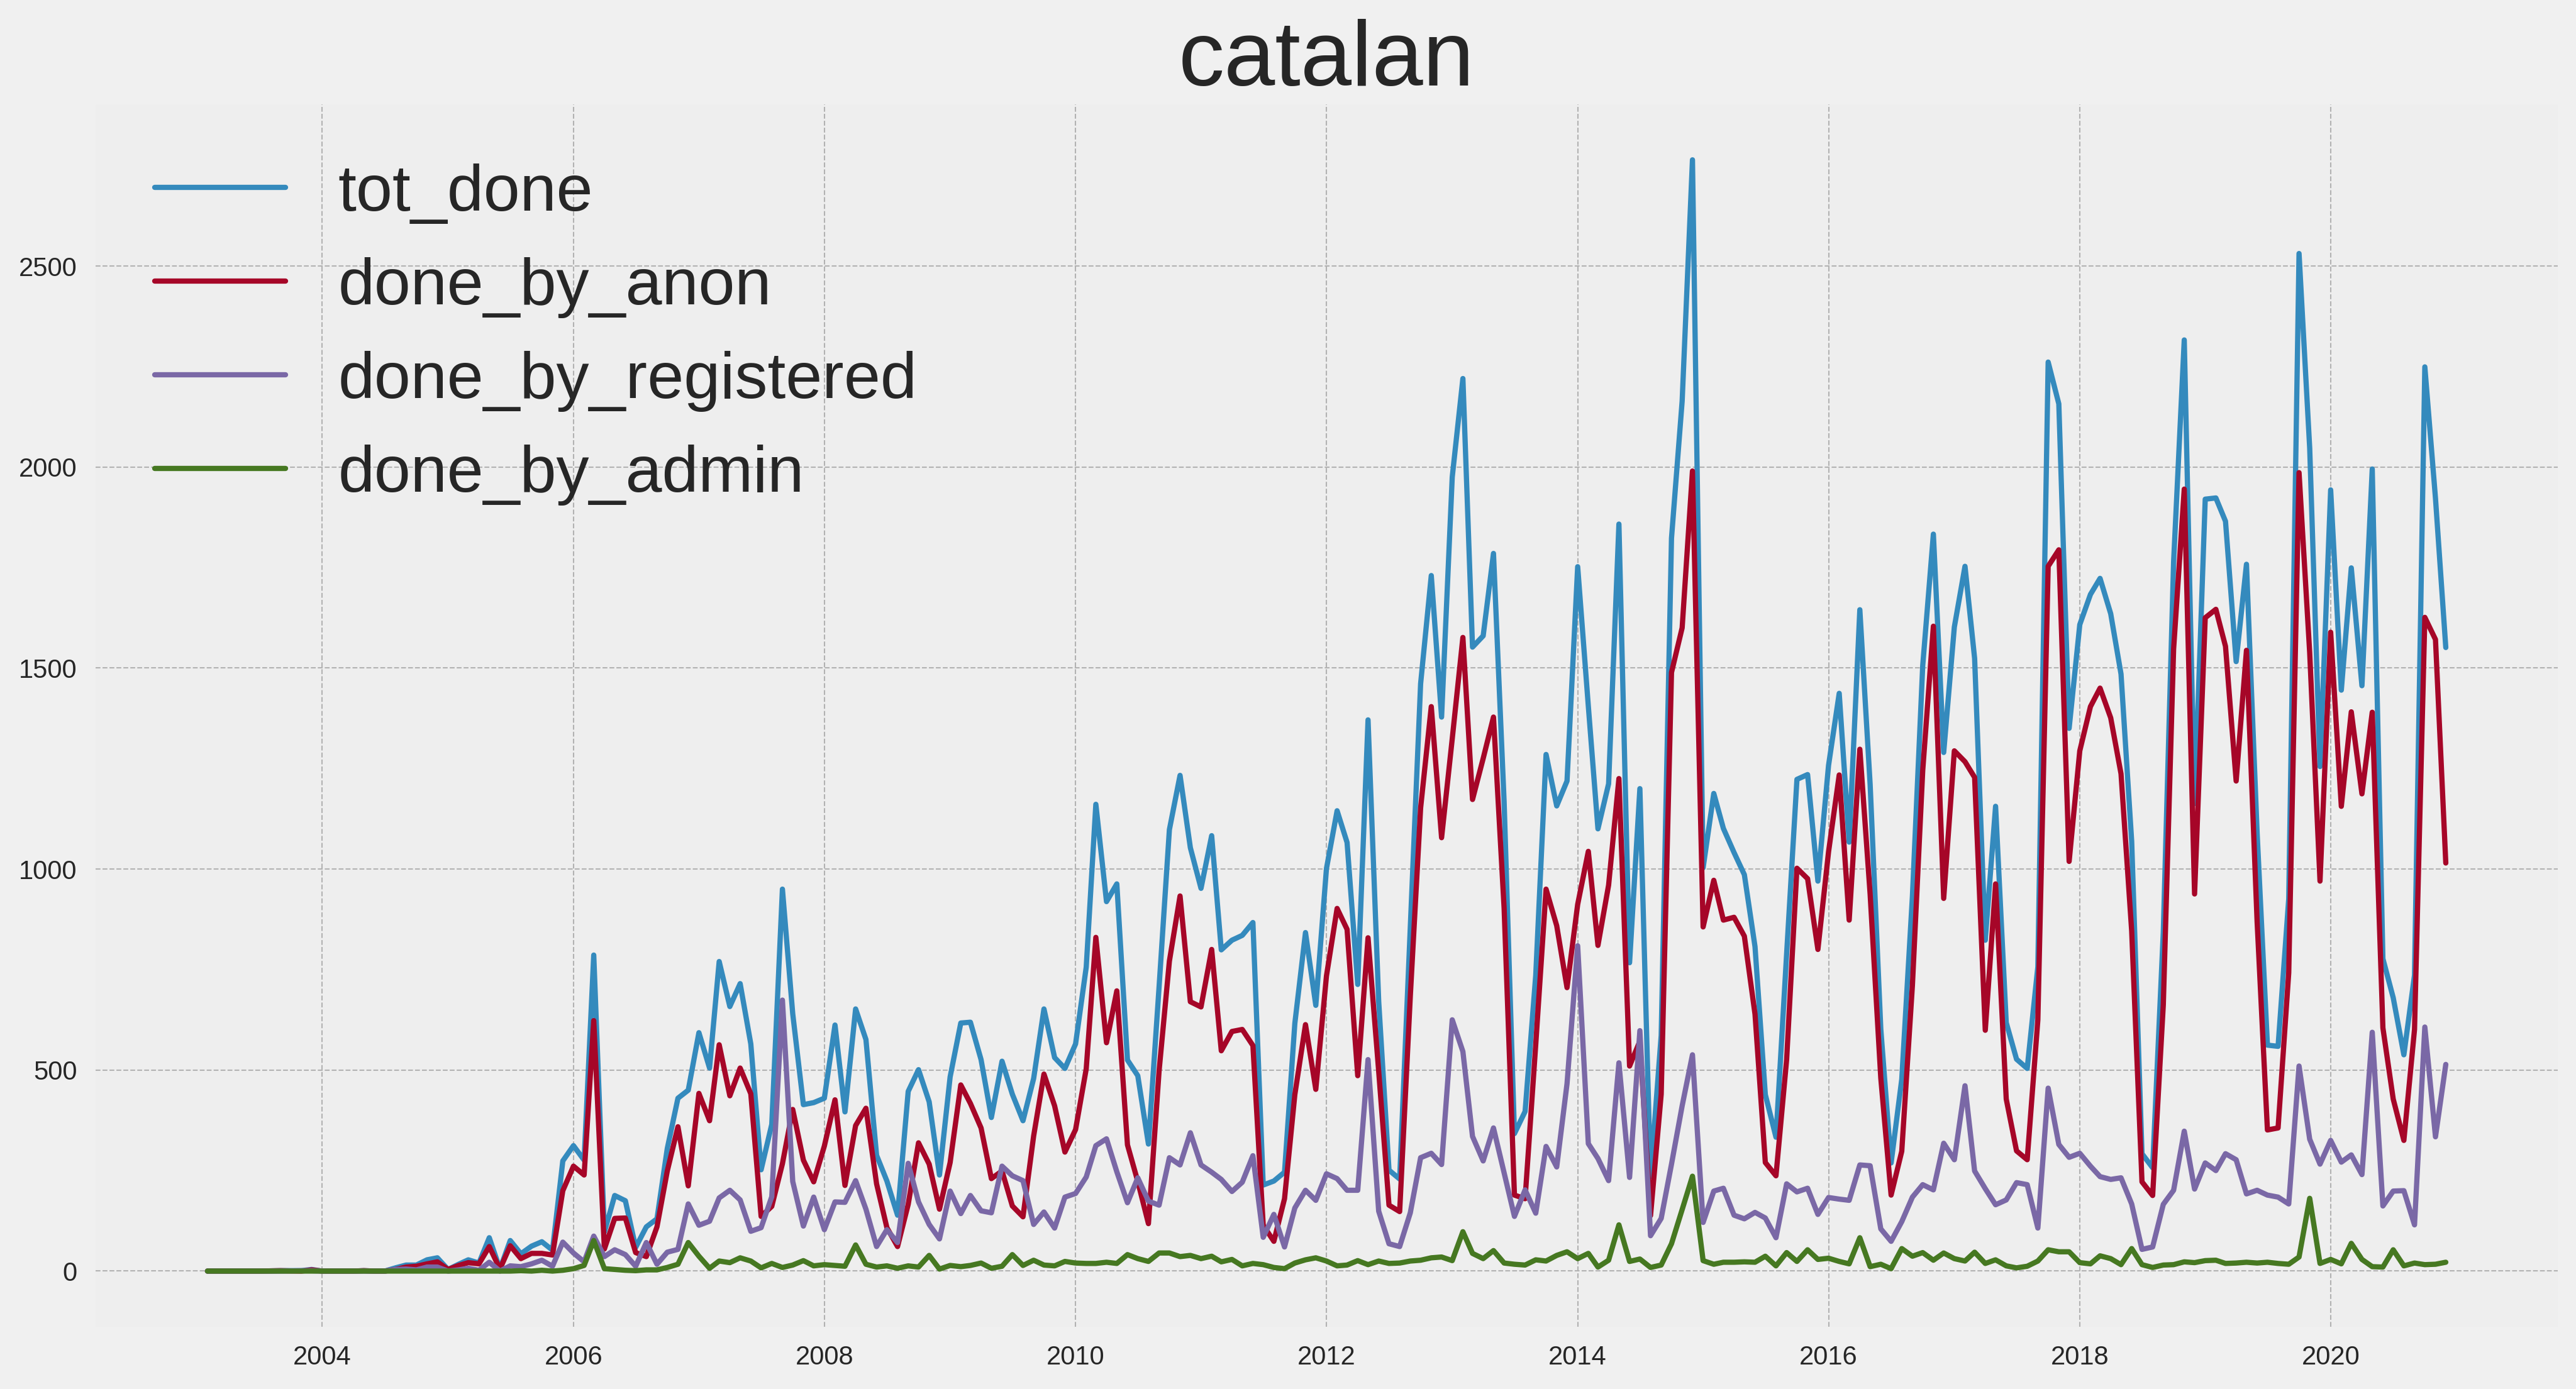
\includegraphics[width=0.49\textwidth]{./chapters/04/assets/revert_done_ca.png}
    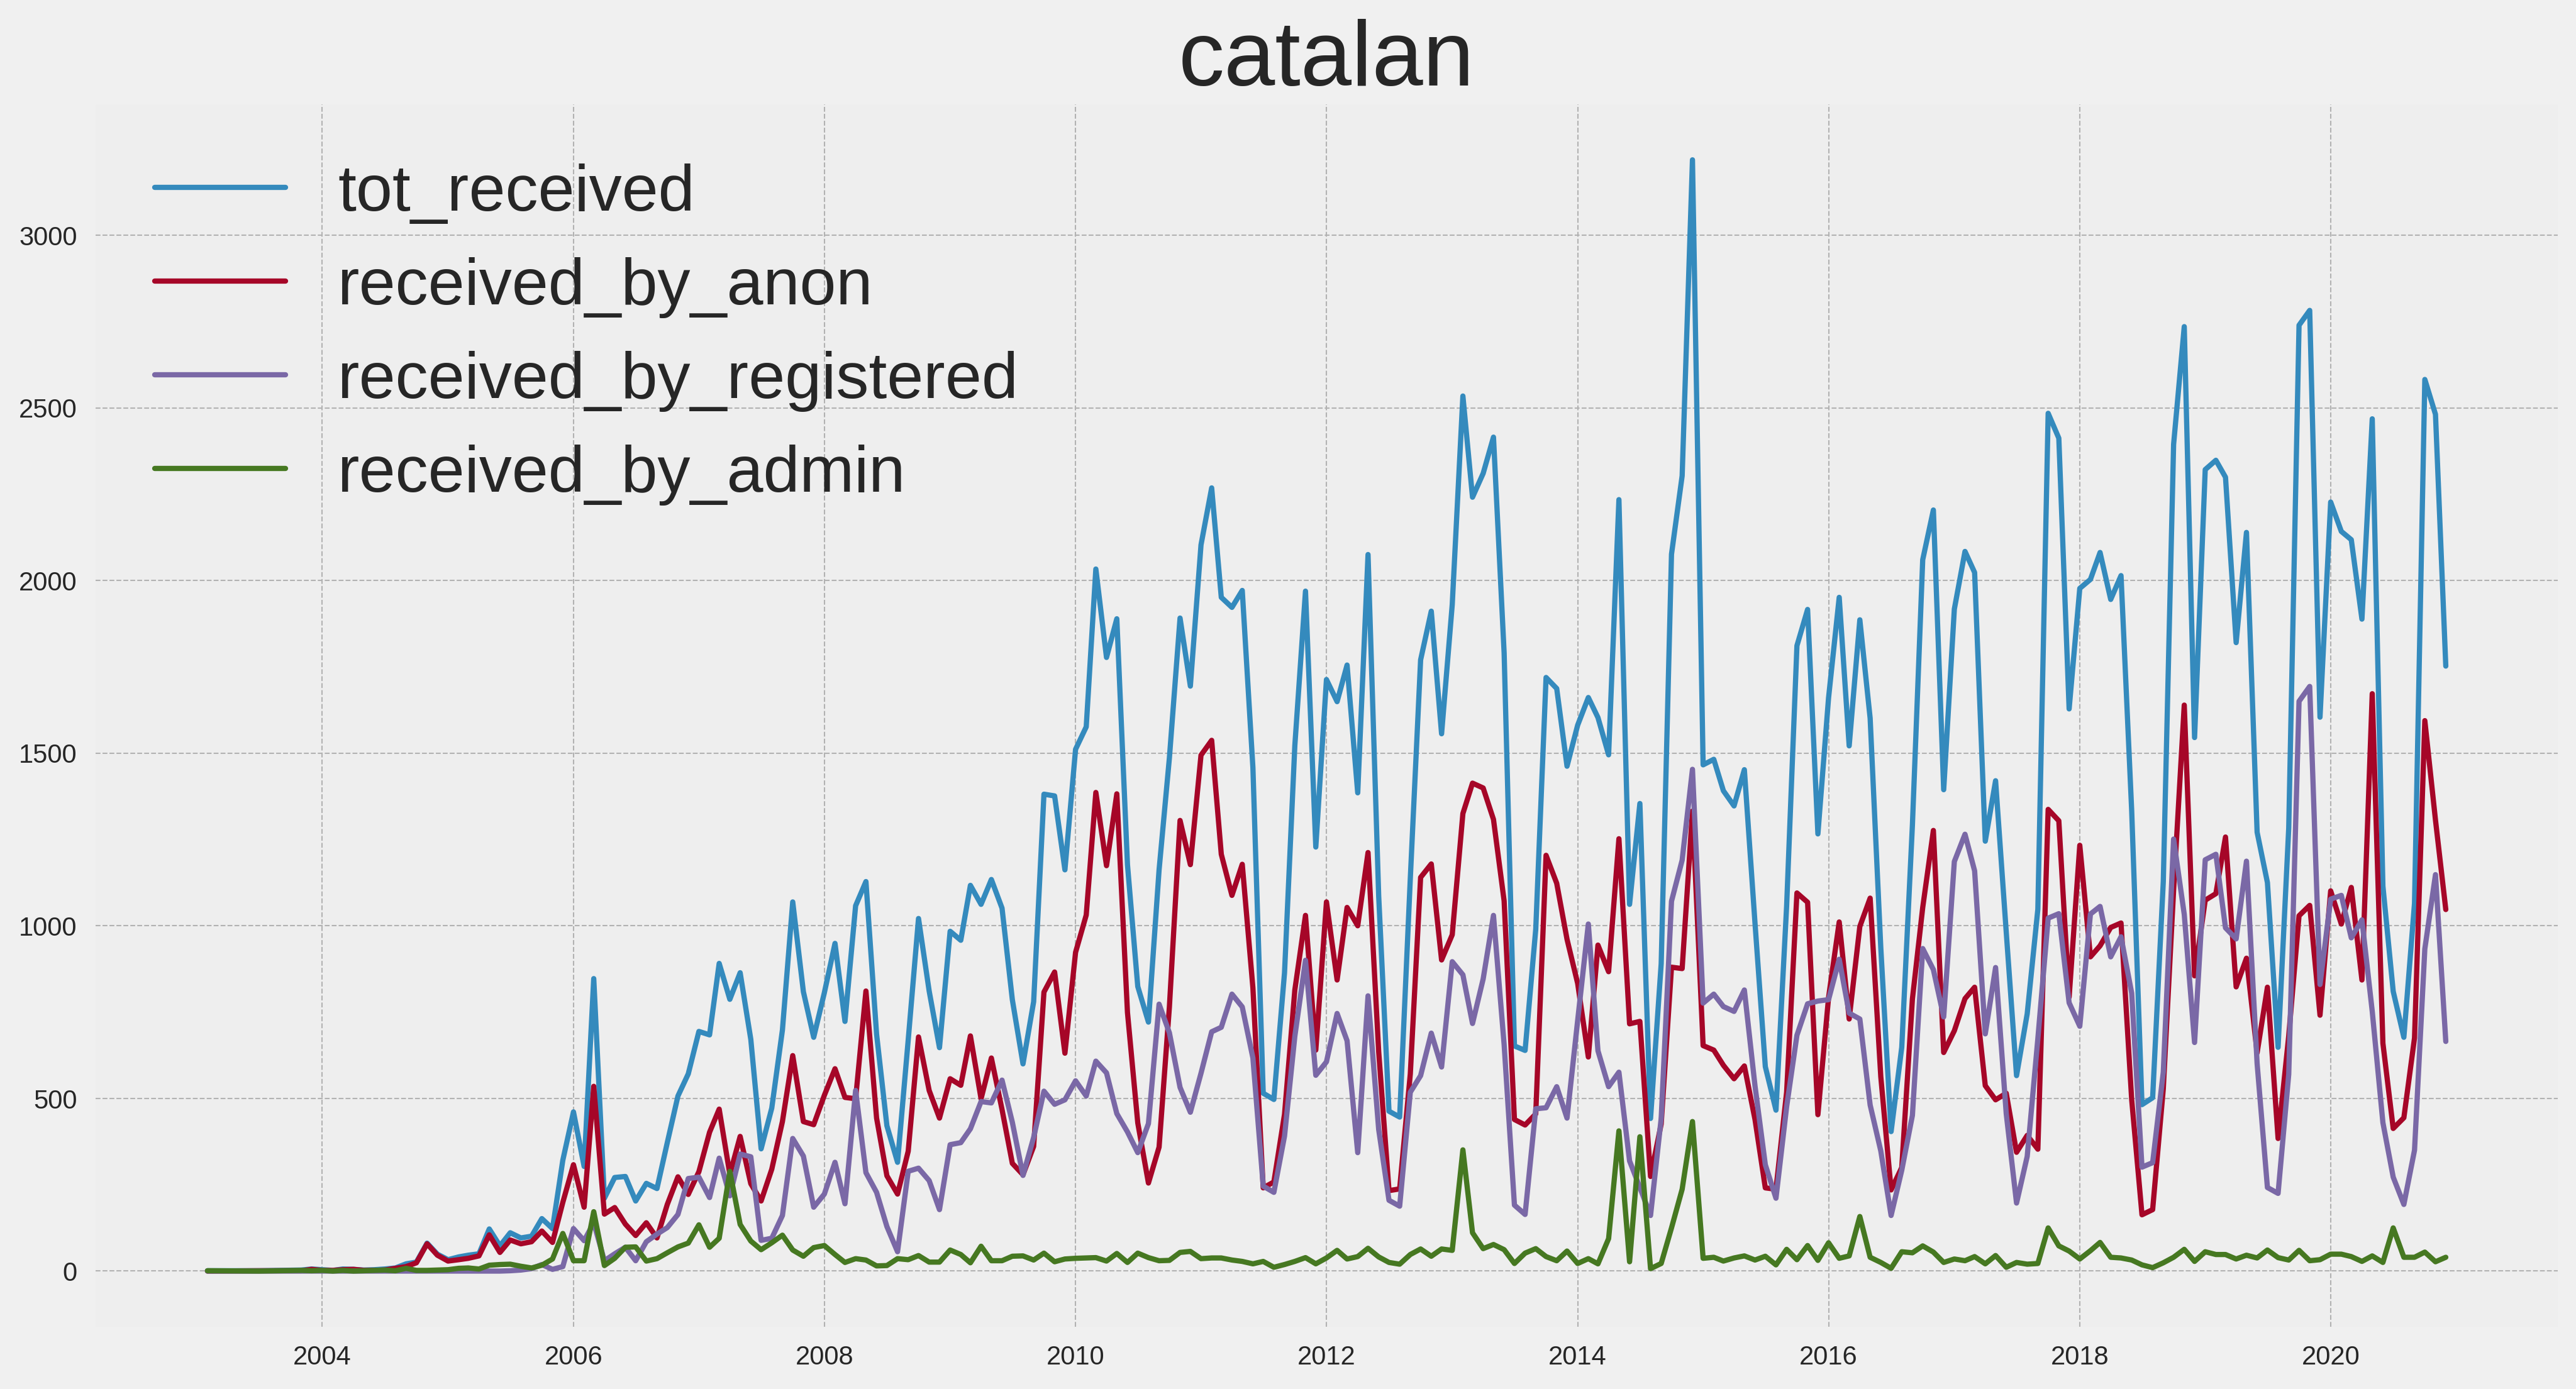
\includegraphics[width=0.49\textwidth]{./chapters/04/assets/revert_received_ca.png}
    \caption{number of chain by month of juan}
    \label{fig:revuser}
\end{figure}








      \chapter{Infrastacture}
all the code in available on Github, there is an onrganiziation called Wiki. in which every team
member commeted theure code so we can gather all this in one place 
for this work we mostly used python. The code has been hosted on the Unitn cricca server 
\subsection{Multi Language}
All the dataset computed are the results of several python scripts launched singularly. All the work
has been done using the italian wikipedia as example. Automatizing the process allow us to run all
the scripts in different languages. For achieving this automatation we used a bash script which
takes the language as parameters e.g ./generate\_dataset it takes the data from the WikiMedia history
dumps in italian, create a folder "it" and all the subfolders needed and generate the dataset in the
right place. the only requirements is that the dump is donwloaded  here the folder structure:  

\dirtree{%
.1 ita.
.2 chains.
.3 user.
.4 wars.json.
.3 page.
.4 wars.json.
.3 month.
.4 page.tsv.
.4 user.tsv.
.3 page\_reg.
.4 wars.json.
.2 group.
.3 user.
.4 mutuals.tsv.
.4 reverts.tsv.
.4 all.tsv.
.3 page.
.4 mutuals.tsv.
.4 reverts.tsv.
.4 all.tsv.
}

      \chapter{Conclusions}
This is still an open project, so the results described in this report are not complete. The largest
portion of the time has been dedicated to the computation of the datasets. For the analysis defined in the project
description we should combine the data of all project members. Nevertheless, with the generated
datasets it is possible to draw some conclusions. We have seen how the language, and so the living place,
of the users, characterizes Wikipedia. We have seen only some languages but the study could be extended
to all the available languages without any problem.\\

Future works will comprehend, besides the studies in different languages, an interactive dashboard
with this data available online and one from the other group members. This allows the users to
dynamically retrieve the data and plot the results as they wish.\\

Wikipedia is full of vandals but fortunately, they are quickly neutralised. From the number of chains we
can understand in which topic which people cannot reach an agreement; in Italy and south
America these topics are sport, especially football, while in Catalunya the most debated topics are about
territorial belonging.



    \endgroup



    \addcontentsline{toc}{chapter}{Bibliografia}
    \bibliographystyle{plain}
    \bibliography{biblio}

    \titleformat{\chapter}
        {\normalfont\Huge\bfseries}{Allegato \thechapter}{1em}{}
    % sezione Allegati - opzionale
    \appendix
    \chapter{Titolo primo allegato}

Lorem ipsum dolor sit amet, consectetur adipiscing elit. Donec sed nunc orci. Aliquam nec nisl vitae sapien pulvinar dictum quis non urna. Suspendisse at dui a erat aliquam vestibulum. Quisque ultrices pellentesque pellentesque. Pellentesque egestas quam sed blandit tempus. Sed congue nec risus posuere euismod. Maecenas ut lacus id mauris sagittis egestas a eu dui. Class aptent taciti sociosqu ad litora torquent per conubia nostra, per inceptos himenaeos. Pellentesque at ultrices tellus. Ut eu purus eget sem iaculis ultricies sed non lorem. Curabitur gravida dui eget ex vestibulum venenatis. Phasellus gravida tellus velit, non eleifend justo lobortis eget. 

\section{Titolo}
Lorem ipsum dolor sit amet, consectetur adipiscing elit. Donec sed nunc orci. Aliquam nec nisl vitae sapien pulvinar dictum quis non urna. Suspendisse at dui a erat aliquam vestibulum. Quisque ultrices pellentesque pellentesque. Pellentesque egestas quam sed blandit tempus. Sed congue nec risus posuere euismod. Maecenas ut lacus id mauris sagittis egestas a eu dui. Class aptent taciti sociosqu ad litora torquent per conubia nostra, per inceptos himenaeos. Pellentesque at ultrices tellus. Ut eu purus eget sem iaculis ultricies sed non lorem. Curabitur gravida dui eget ex vestibulum venenatis. Phasellus gravida tellus velit, non eleifend justo lobortis eget. 

\subsection{Sottotitolo}
Lorem ipsum dolor sit amet, consectetur adipiscing elit. Donec sed nunc orci. Aliquam nec nisl vitae sapien pulvinar dictum quis non urna. Suspendisse at dui a erat aliquam vestibulum. Quisque ultrices pellentesque pellentesque. Pellentesque egestas quam sed blandit tempus. Sed congue nec risus posuere euismod. Maecenas ut lacus id mauris sagittis egestas a eu dui. Class aptent taciti sociosqu ad litora torquent per conubia nostra, per inceptos himenaeos. Pellentesque at ultrices tellus. Ut eu purus eget sem iaculis ultricies sed non lorem. Curabitur gravida dui eget ex vestibulum venenatis. Phasellus gravida tellus velit, non eleifend justo lobortis eget. 


\chapter{Titolo secondo allegato}

Lorem ipsum dolor sit amet, consectetur adipiscing elit. Donec sed nunc orci. Aliquam nec nisl vitae sapien pulvinar dictum quis non urna. Suspendisse at dui a erat aliquam vestibulum. Quisque ultrices pellentesque pellentesque. Pellentesque egestas quam sed blandit tempus. Sed congue nec risus posuere euismod. Maecenas ut lacus id mauris sagittis egestas a eu dui. Class aptent taciti sociosqu ad litora torquent per conubia nostra, per inceptos himenaeos. Pellentesque at ultrices tellus. Ut eu purus eget sem iaculis ultricies sed non lorem. Curabitur gravida dui eget ex vestibulum venenatis. Phasellus gravida tellus velit, non eleifend justo lobortis eget. 

\section{Titolo}
Lorem ipsum dolor sit amet, consectetur adipiscing elit. Donec sed nunc orci. Aliquam nec nisl vitae sapien pulvinar dictum quis non urna. Suspendisse at dui a erat aliquam vestibulum. Quisque ultrices pellentesque pellentesque. Pellentesque egestas quam sed blandit tempus. Sed congue nec risus posuere euismod. Maecenas ut lacus id mauris sagittis egestas a eu dui. Class aptent taciti sociosqu ad litora torquent per conubia nostra, per inceptos himenaeos. Pellentesque at ultrices tellus. Ut eu purus eget sem iaculis ultricies sed non lorem. Curabitur gravida dui eget ex vestibulum venenatis. Phasellus gravida tellus velit, non eleifend justo lobortis eget. 

\subsection{Sottotitolo}
Lorem ipsum dolor sit amet, consectetur adipiscing elit. Donec sed nunc orci. Aliquam nec nisl vitae sapien pulvinar dictum quis non urna. Suspendisse at dui a erat aliquam vestibulum. Quisque ultrices pellentesque pellentesque. Pellentesque egestas quam sed blandit tempus. Sed congue nec risus posuere euismod. Maecenas ut lacus id mauris sagittis egestas a eu dui. Class aptent taciti sociosqu ad litora torquent per conubia nostra, per inceptos himenaeos. Pellentesque at ultrices tellus. Ut eu purus eget sem iaculis ultricies sed non lorem. Curabitur gravida dui eget ex vestibulum venenatis. Phasellus gravida tellus velit, non eleifend justo lobortis eget. 




\end{document}


%%%%%%%%%%%%%%%%%%%%%%%%%%%%%%%%%%%%%%%%%%%%%%%%%%%%%%%%%%%%%%%%%%%%%%%%%%
%%%%%%%%%%%%%%%%%%%%%%%%%%%%%%%%%%%%%%%%%%%%%%%%%%%%%%%%%%%%%%%%%%%%%%%%%%
%% Nota
%%%%%%%%%%%%%%%%%%%%%%%%%%%%%%%%%%%%%%%%%%%%%%%%%%%%%%%%%%%%%%%%%%%%%%%%%%
%% Si ricorda che il numero massimo di facciate e' 30.
%% Nel conteggio delle facciate sono incluse 
%%   indice
%%   sommario
%%   capitoli
%% Dal conteggio delle facciate sono escluse
%%   frontespizio
%%   ringraziamenti
%%   allegati    
%%%%%%%%%%%%%%%%%%%%%%%%%%%%%%%%%%%%%%%%%%%%%%%%%%%%%%%%%%%%%%%%%%%%%%%%%%
%%%%%%%%%%%%%%%%%%%%%%%%%%%%%%%%%%%%%%%%%%%%%%%%%%%%%%%%%%%%%%%%%%%%%%%%%%
%%%%%%%%%%%%%%%%%%%%%%%%%%%%%%%%%%%%%%%%%%%%%%%%%%%%%%%%%%%%%%%%%%%%%%%%%%
%%%%%%%%%%%%%%%%%%%%%%%%%%%%%%%%%%%%%%%%%%%%%%%%%%%%%%%%%%%%%%%%%%%%%%%%%%
%% Nota
%%%%%%%%%%%%%%%%%%%%%%%%%%%%%%%%%%%%%%%%%%%%%%%%%%%%%%%%%%%%%%%%%%%%%%%%%%
%% Nella bibliografia devono essere riportati tutte le fonti consultate 
%% per lo svolgimento della tesi. La bibliografia deve essere redatta 
%% in ordine alfabetico sul cognome del primo autore. 
%% 
%% La forma della citazione bibliografica va inserita secondo la fonte utilizzata:
%% 
%% LIBRI
%% Cognome e iniziale del nome autore/autori, la data di edizione, titolo, casa editrice, eventuale numero dell’edizione. 
%% 
%% ARTICOLI DI RIVISTA
%% Cognome e iniziale del nome autore/autori, titolo articolo, titolo rivista, volume, numero, numero di pagine.
%% 
%% ARTICOLI DI CONFERENZA
%% Cognome e iniziale del nome autore/autori (anno), titolo articolo, titolo conferenza, luogo della conferenza (città e paese), date della conferenza, numero di pagine. 
%% 
%% SITOGRAFIA
%% La sitografia contiene un elenco di indirizzi Web consultati e disposti in ordine alfabetico. 
%% E’ necessario:
%%   Copiare la URL (l’indirizzo web) specifica della pagina consultata
%%   Se disponibile, indicare il cognome e nome dell’autore, il titolo ed eventuale sottotitolo del testo
%%   Se disponibile, inserire la data di ultima consultazione della risorsa (gg/mm/aaaa).    
%%%%%%%%%%%%%%%%%%%%%%%%%%%%%%%%%%%%%%%%%%%%%%%%%%%%%%%%%%%%%%%%%%%%%%%%%%
%%%%%%%%%%%%%%%%%%%%%%%%%%%%%%%%%%%%%%%%%%%%%%%%%%%%%%%%%%%%%%%%%%%%%%%%%%
    
